\documentclass[letterpaper]{article}
\usepackage[submission]{aaai2027}
\usepackage{times}
\usepackage{helvet}
\usepackage{courier}
\usepackage[hyphens]{url}
\usepackage{graphicx}
\urlstyle{rm}
\def\UrlFont{\rm}
\usepackage{natbib}
\frenchspacing
\setlength{\emergencystretch}{2em}
\raggedbottom

% More permissive float placement for the supplementary material.
\setcounter{topnumber}{6}
\setcounter{bottomnumber}{4}
\setcounter{totalnumber}{10}
\renewcommand{\topfraction}{0.97}
\renewcommand{\bottomfraction}{0.90}
\renewcommand{\textfraction}{0.03}
\renewcommand{\floatpagefraction}{0.82}
\renewcommand{\dbltopfraction}{0.97}
\renewcommand{\dblfloatpagefraction}{0.82}
\setlength{\pdfpagewidth}{8.5in}
\setlength{\pdfpageheight}{11in}

\usepackage{algorithm}
\usepackage{algorithmic}
\usepackage{amsmath}
\usepackage{amssymb}
\usepackage{amsfonts}
\usepackage{booktabs}
\usepackage{array}
\usepackage{placeins}
\usepackage{dblfloatfix}
\usepackage{balance}

\pdfinfo{
/TemplateVersion (2027.1)
}
\setcounter{secnumdepth}{0}

\newcommand{\method}{\textsc{TA-DVFG}}
\newcommand{\Gc}{\mathcal{G}_c}
\newcommand{\Ec}{\mathcal{E}_c}
\newcommand{\Ni}{\mathcal{N}_i}
\newcommand{\R}{\mathbb{R}}
\newtheorem{proposition}{Proposition}

\title{Supplementary Material: Collaboration without Representation Alignment: Sparse Prediction Topology Learning for Vertical Graph Views}
\author{Anonymous Submission}
\affiliations{}

\begin{document}
\maketitle

\renewcommand{\thetable}{S\arabic{table}}
\renewcommand{\thefigure}{S\arabic{figure}}
\renewcommand{\theequation}{S\arabic{equation}}
\renewcommand{\thealgorithm}{S\arabic{algorithm}}
\renewcommand{\theproposition}{S\arabic{proposition}}

\section{Supplementary Overview}

This document contains supporting material for the main paper. It keeps six
evaluation regimes explicit: (i) the shuffled HGB cached-core suite used for
the primary controlled comparison, (ii) the fresh within-suite ACM Hard
latent-alignment reference study, (iii) the MovieLens suite with explicitly
heterogeneous local predictors and 15-party weak-predictor stress settings,
(iv) the active-party label-location suite, (v) nested HGB weak-party scaling
with a fixed useful-predictor set, and (vi) consensus-depth sensitivity for
multi-hop propagation. It additionally reports mechanism audits that separate
participant selection, degree-dependent readout weighting, and peer exchange.
Global diagnostic and latent-fusion references use stronger centralized
information and are not deployable sparse P2P topology baselines.

\method{} is an inference-stage topology/readout mechanism layered over
independently trained local predictors. At each scheduled refresh, a
low-frequency active party uses held-out validation predictions to recompute the
topology; the selector does not back-propagate into local models. The graph has
two deployment roles: it determines which predictors participate in active
readout, and its selected links carry peer prediction messages for party-local
inference. An active-party readout additionally collects the post-consensus
predictions that it consumes, whereas party-local readout requires no global
collection. The mechanism audits show that direct subset selection is a strong
lower-cost alternative for active-only deployment, while peer exchange
materially improves connected parties' local predictions. The method does not
provide a formal privacy guarantee and is not presented as a fully serverless
end-to-end VFGL protocol. The MovieLens 15-party Main and Hard settings are
controlled stress constructions rather than naturally occurring
15-organization federations.

\section{Evaluation Questions and Construction Details}

The experiments are organized around five questions: \textbf{Q1}, whether
learned sparsity improves over dense, communication-matched, and
no-collaboration references; \textbf{Q2}, whether the approach transfers to
explicitly heterogeneous real-world predictors; \textbf{Q3}, what graph
structure provides beyond direct participant selection and edge-local
adaptation; \textbf{Q4}, whether different deployment readouts require
different topologies; and \textbf{Q5}, how sparse prediction-space
collaboration compares with stronger-information latent-alignment interfaces
when genuine hidden states can be exported from identical frozen local
predictors. The main-paper evidence is the HGB comparison for Q1, the MovieLens
evidence for Q2, the mechanism audits for Q3--Q4, and the ACM Hard five-seed
alignment-reference study for Q5.

\paragraph{Controlled HGB construction.}
All parties classify the same aligned target nodes under the original HGB labels
and the same dataset-level train/validation/test split; the controlled
construction changes only each party's private feature/graph view. Useful
predictors are instantiated from dataset-specific relation or KNN graph views.
ACM uses PAP, PSP, and KNN views; DBLP uses APA, APCPA, APTPA, and KNN; IMDB
uses MAM, MDM, and KNN.

Weak/noisy predictors are controlled distractors rather than relabeled tasks.
For each weak/noisy party and seed, the private feature block is first permuted
across target rows using a seed-specific row permutation and is then perturbed
with zero-mean Gaussian noise of scale $1.0$. The party's private graph is
replaced by an independently sampled random graph with configured degree $4$.
Labels and train/validation/test membership are never changed by this
construction. Main uses six useful and nine controlled weak/noisy predictors;
Hard uses three useful and twelve controlled weak/noisy predictors. Party
identities are reshuffled independently for every seed so that \method{} cannot
exploit a fixed party index, and all compared methods receive the same cached
local-prediction trajectories. This design isolates collaboration and topology
effects rather than differences in target definition, data splitting, or local
training runs.

\paragraph{Nested weak-party scaling.}
To isolate the effect of weak-predictor population size from the fixed
Main/Hard endpoints, we keep three useful predictors fixed within each seed
and incrementally add 0, 2, 5, 10, or 15 weak predictors. This produces nested
3-, 5-, 8-, 13-, and 18-party settings on ACM and DBLP. The design therefore
measures how each collaboration mechanism changes as weak predictors are added
to the same useful-predictor core rather than comparing only two independently
constructed stress endpoints.

\paragraph{Consensus-depth sensitivity.}
To test whether the one-step default reduces the selected graph to independent
pairwise interactions, we rerun topology selection separately for
$K\in\{1,2,3\}$ on ACM and DBLP Hard using identical cached local predictors
and all other selector defaults. We report both predictive performance and
$K$-hop reachability.

\paragraph{MovieLens task and party interfaces.}
We use the GroupLens MovieLens 1M release (\texttt{ml-1m.zip}). The prediction
targets are the observed rating rows themselves: this is not implicit-feedback
link prediction, and unobserved user--item pairs are never introduced as
negatives. An observed row is positive when its rating is at least $4$ and
negative when its rating is in $\{1,2,3\}$; no negative sampling is used.

For deterministic splitting, rating rows are ordered lexicographically by
\texttt{(timestamp, user\_id, movie\_id)} and then divided chronologically into
70\% train, 10\% validation, and 20\% test partitions. The resulting ordered
user--item rating rows form the common aligned target index used by all five
parties. Each party receives a distinct private view and independently designed
predictor family, but every party scores exactly the same aligned target rows.
The topology method sees only task-level prediction scores.

All trainable local predictors and fitted preprocessing statistics are estimated
from the training partition only. This includes matrix-factorization state,
local predictor parameters, popularity, mean-rating, positive-rate and count
statistics, and the mean and standard deviation used for timestamp
normalization. Validation labels are used only for reliability estimation and
topology selection; test labels are reserved for final reporting. For binary
recommendation, a positive-class probability $p_i[v]$ is represented as the
compatible two-class vector $(1-p_i[v],p_i[v])$, so the same prediction-space
consensus applies. The five interfaces are listed in
Table~\ref{tab:supp-movielens-interfaces}.

\section{Algorithmic Details}

\subsection{Reliability, Consensus, and Readouts}

Let $\mathcal{M}(\cdot,\cdot)\in[0,1]$ denote the task-level validation
metric: classification accuracy for HGB and ROC-AUC for MovieLens. For
MovieLens, each scalar positive-class probability is represented as
$(1-p,p)$, so all exchanged predictions lie in a common two-class simplex.
For topology-validation targets $\mathcal{V}_{\mathrm{topo}}$, party $i$ has
reliability
\begin{equation}
r_i=\mathcal{M}\!\left(
P_i[\mathcal{V}_{\mathrm{topo}}],
y_{\mathcal{V}_{\mathrm{topo}}}
\right),
\qquad
\bar r_i=\max(r_i,10^{-3}).
\end{equation}
The implemented reliability exponent is $1.0$. For a candidate topology $E$,
initialize $P_i^{(0)}(E)=P_i$. For a non-isolated party, define
\begin{equation}
\alpha_{ij}(E)=
\frac{\bar r_j}
{\sum_{\ell\in\Ni(E)}\bar r_\ell},
\qquad j\in\Ni(E),
\end{equation}
and update
\begin{equation}
P_i^{(k+1)}(E)=
\eta P_i^{(k)}(E)
+(1-\eta)\sum_{j\in\Ni(E)}
\alpha_{ij}(E)P_j^{(k)}(E).
\end{equation}
Isolated parties retain their current prediction. The reported configuration
uses one consensus step and self-weight $\eta=0.85$.

The topology affects deployment through two distinct mechanisms. First, it
determines the active-readout participant set and topology-dependent weights.
Second, when $K>0$, it defines the peer links over which predictions are
exchanged. For active-party readout, define
\begin{equation}
\mathcal{S}(E)=
\begin{cases}
\{i:\deg_E(i)>0\}, & E\neq\emptyset,\\
\{1,\ldots,N\}, & E=\emptyset.
\end{cases}
\end{equation}
Thus, non-isolated parties are read out when the topology contains at least one
edge, and the edgeless topology falls back to all parties. The active party has
no additional special term. For $i\in\mathcal{S}(E)$, the implemented readout
weight is
\begin{equation}
\omega_i(E)=
\bar r_i\bigl(\deg_E(i)+1\bigr)^{1/2},
\end{equation}
and
\begin{equation}
Q_{\mathrm{active}}(E)=
\sum_{i\in\mathcal{S}(E)}
\frac{\omega_i(E)}
{\sum_{j\in\mathcal{S}(E)}\omega_j(E)}
P_i^{(K)}(E).
\end{equation}
The deployment objectives use the same task metric:
\begin{align}
s_{\mathrm{active}}(E)&=\mathcal{M}\!\left(
Q_{\mathrm{active}}(E)[\mathcal{V}_{\mathrm{topo}}],
 y_{\mathcal{V}_{\mathrm{topo}}}\right),\nonumber\\
s_{\mathrm{local}}(E)&=\frac{1}{N}\sum_{i=1}^{N}
\mathcal{M}\!\left(P_i^{(K)}(E)[\mathcal{V}_{\mathrm{topo}}],
 y_{\mathcal{V}_{\mathrm{topo}}}\right),\nonumber\\
s_{\mathrm{joint}}(E)&=\lambda s_{\mathrm{active}}(E)
+(1-\lambda)s_{\mathrm{local}}(E).
\end{align}

\subsection{Greedy Topology Selection}

The constrained argmax in the main paper defines a conceptual optimum
$E^\star$. Algorithm~\ref{alg:supp-topology} is a greedy approximation and
returns a feasible topology $\widehat E$; no global-optimality claim is made.

Unless otherwise stated, the candidate set is the complete undirected graph over
the $N$ parties,
$\Ec=\{\{i,j\}:1\le i<j\le N\}$.
Let
\begin{equation}
\begin{aligned}
\mathcal{F}(E)=\bigl\{e\in\Ec\setminus E:\;&
|E\cup\{e\}|\le B,\;\\
&\deg_{E\cup\{e\}}(i)\le d_{\max}\ \forall i
\bigr\}.
\end{aligned}
\end{equation}
Each feasible extension is scored by running the complete consensus-and-readout
pipeline on $E\cup\{e\}$.

\begin{algorithm}[t]
\caption{Validation-Assisted Sparse Topology Learning}
\label{alg:supp-topology}
\begin{algorithmic}[1]
\REQUIRE Validation predictions $\{P_i\}$, labels
$y_{\mathcal{V}_{\mathrm{topo}}}$, reliabilities $\{r_i\}$,
objective $s(\cdot)$, edge budget $B$, degree limit $d_{\max}$,
minimum links $m$, threshold $\tau$
\STATE $E\leftarrow\emptyset$; $q\leftarrow s(E)$
\WHILE{$|E|<B$}
\STATE Construct $\mathcal{F}(E)$
\IF{$\mathcal{F}(E)=\emptyset$}
\STATE \textbf{break}
\ENDIF
\FORALL{$e\in\mathcal{F}(E)$}
\STATE Run consensus and compute $q_e\leftarrow s(E\cup\{e\})$
\ENDFOR
\STATE $e^\star\leftarrow\arg\max_{e\in\mathcal{F}(E)} q_e$
\IF{$|E|<m$ or $q_{e^\star}-q\ge\tau$}
\STATE $E\leftarrow E\cup\{e^\star\}$; $q\leftarrow q_{e^\star}$
\ELSE
\STATE \textbf{break}
\ENDIF
\ENDWHILE
\RETURN $\widehat E\leftarrow E$
\end{algorithmic}
\end{algorithm}

For deterministic reproduction, candidates are ordered by descending pairwise
utility and then by descending party indices. If two candidate extensions have
the same graph-level validation score, the candidate with higher pairwise
utility is preferred; exact utility ties retain the first candidate in this
deterministic order. The minimum-link parameter $m$ forces only the initial
$m$ additions. For $m=0$, even the first edge must improve the validation
objective by at least $\tau$, so an empty graph is permitted. Thereafter, the
search stops when no feasible extension clears $\tau$; $B$ remains an upper
bound rather than a required edge count.

\subsection{Optional Label-Location Training Variant}

For the stricter label-location setting, only active-party training code directly
receives $y_{\mathcal{T}}$. Passive party $i$ sends train-node logits
$Z_i[\mathcal{T}]$ to the active party. The active party evaluates
\begin{equation}
L_i=\operatorname{CE}(Z_i[\mathcal{T}],y_{\mathcal{T}})
\end{equation}
and returns
\begin{equation}
G_i=\frac{\partial L_i}{\partial Z_i[\mathcal{T}]}.
\end{equation}
Party $i$ back-propagates $G_i$ through its private model. The label values do
not enter passive-party code directly. This separates the location of direct
label access but does not establish label confidentiality: exact logit gradients
can reveal label information. The protocol is therefore neither cryptographic
nor differential-private.

\subsection{Communication Accounting}

Label-location training communicates
$2(N-1)|\mathcal{T}|C$ scalars per epoch. One topology update collects at most
$N|\mathcal{V}_{\mathrm{topo}}|C$ validation-prediction scalars. For $M$
inference targets and $K$ consensus steps, peer exchange costs
\begin{equation}
2|\widehat E|KMC.
\end{equation}
If every party has degree at most $d_{\max}$, then
$2|\widehat E|\le Nd_{\max}$ and peer exchange is bounded by
$Nd_{\max}KMC$, compared with $N(N-1)KMC$ for Full Mesh. Party-local readout
needs no additional global collection. To match the benchmark accounting used
in the main paper, readout payload counts every prediction vector consumed by
the readout: $|\mathcal{S}(\widehat E)|MC$ for the active readout, $NMC$ for
Global Uniform or Reliability Vote, and $kMC$ for Global Top-$k$. Peer exchange
counts actual transmitted scalars; readout payload is reported separately.

\section{Basic Properties and Proofs}

\begin{proposition}[Feasibility and termination]
Algorithm~\ref{alg:supp-topology} returns a topology
$\widehat E\subseteq\Ec$ satisfying $|\widehat E|\le B$ and
$\deg_{\widehat E}(i)\le d_{\max}$ for every party $i$. It terminates after at
most $B$ accepted edge additions.
\end{proposition}

\paragraph{Proof.}
The initial graph is $E_0=\emptyset$, which satisfies both
$|E_0|\le B$ and $\deg_{E_0}(i)=0\le d_{\max}$ for all $i$. Suppose the current
graph $E_t$ is feasible. Algorithm~\ref{alg:supp-topology} may add only an edge
$e\in\mathcal{F}(E_t)$. By definition of $\mathcal{F}(E_t)$,
$|E_t\cup\{e\}|\le B$ and
$\deg_{E_t\cup\{e\}}(i)\le d_{\max}$ for every $i$. Hence feasibility is
preserved by induction after every accepted update. Each accepted iteration
adds exactly one previously absent edge, so after at most $B$ accepted updates
the edge-budget condition prevents any further addition. The algorithm may stop
earlier if $\mathcal{F}(E)=\emptyset$ or if the validation-gain condition fails.
Therefore the returned graph is feasible and the procedure terminates after at
most $B$ accepted edge additions. \hfill$\square$

\begin{proposition}[Simplex preservation]
Assume every local predictor maps each target to the same class simplex
$\Delta^C$. Then every consensus update is well defined regardless of private
encoder architecture or hidden dimension. Moreover, if
$P_i^{(0)}[v]\in\Delta^C$ for every party $i$ and target $v$, then
$P_i^{(k)}[v]\in\Delta^C$ for every $k\ge0$.
\end{proposition}

\paragraph{Proof.}
The consensus rule combines only vectors in $\R^C$; it never adds, multiplies,
or compares private hidden representations. Thus heterogeneous latent spaces do
not affect dimensional compatibility of the update. For a fixed non-isolated
receiver $i$, the neighbor weights satisfy $\alpha_{ij}(E)\ge0$ because
$\bar r_j\ge10^{-3}>0$, and
\[
\sum_{j\in\Ni(E)}\alpha_{ij}(E)=1.
\]
Because $0\le\eta\le1$, the complete update assigns nonnegative coefficients
$\eta$ to the self prediction and $(1-\eta)\alpha_{ij}$ to each neighbor, whose
sum is
\[
\eta+(1-\eta)\sum_{j\in\Ni(E)}\alpha_{ij}=1.
\]
Assume $P_i^{(k)}[v]\in\Delta^C$ and
$P_j^{(k)}[v]\in\Delta^C$ for every $j\in\Ni(E)$. Then each coordinate of the
update is nonnegative, and
\[
\mathbf{1}^{\top}P_i^{(k+1)}[v]
=\eta+(1-\eta)\sum_{j\in\Ni(E)}\alpha_{ij}=1.
\]
For isolated parties the prediction is unchanged. Hence
$P_i^{(k+1)}[v]\in\Delta^C$. The claim follows for all $k$ by induction from
the valid initial distributions. \hfill$\square$

\begin{proposition}[$K$-hop influence]
Condition on a fixed selected topology $E$ and fixed reliability weights. After
$K$ consensus steps, the prediction $P_i^{(K)}(E)$ can depend only on initial
predictions from parties whose graph distance from $i$ is at most $K$.
\end{proposition}

\paragraph{Proof.}
Conditioning on $E$ and the reliability weights fixes all mixing coefficients.
Let $\mathcal{B}_K(i)$ denote the parties within $K$ hops of $i$ in $E$. For
$K=0$, $P_i^{(0)}$ depends only on party $i$, so the claim holds because
$\mathcal{B}_0(i)=\{i\}$. Assume that for some $K=k$, every
$P_j^{(k)}$ depends only on initial predictions from $\mathcal{B}_k(j)$. The
next update of party $i$ uses only $P_j^{(k)}$ for
$j\in\{i\}\cup\Ni(E)$. Any party in $\mathcal{B}_k(j)$ for such a party $j$ is
at distance at most $k+1$ from $i$. Therefore $P_i^{(k+1)}$ depends only on
initial predictions from $\mathcal{B}_{k+1}(i)$. Induction proves the result.
\hfill$\square$

\begin{proposition}[Sparse communication bound]
For $M$ inference targets and $K$ consensus steps, bidirectional peer exchange
over an undirected selected topology $\widehat E$ communicates
$2|\widehat E|KMC$ scalars. If $\deg_{\widehat E}(i)\le d_{\max}$ for all $i$, then
this cost is at most $Nd_{\max}KMC$. Full Mesh communicates
$N(N-1)KMC$ scalars.
\end{proposition}

\paragraph{Proof.}
At one consensus step, each undirected edge carries one $M\times C$ prediction
matrix in each direction, for $2MC$ transmitted scalars. Repeating this over
$|\widehat E|$ edges and $K$ steps gives $2|\widehat E|KMC$. By the handshake lemma,
\[
2|\widehat E|=\sum_{i=1}^{N}\deg_{\widehat E}(i)\le Nd_{\max},
\]
which yields the bound $Nd_{\max}KMC$. In Full Mesh,
$|E|=N(N-1)/2$, so substituting into the exact peer-exchange expression gives
$N(N-1)KMC$. \hfill$\square$

These results establish feasibility, finite termination, compatibility with
heterogeneous private predictors, probability validity, propagation locality,
and sparse communication scaling. They do not imply global topology optimality,
formal privacy, or convergence of private non-convex local models.

\section{Full HGB Cached-Core Results}

The cached-core suite fixes local graph-view predictors, reshuffles useful/noisy
party positions by seed, and gives every method the same cached local-prediction
trajectories. Table~\ref{tab:supp-complete} reports the complete 13-method
comparison used to support the main-paper HGB claims. The full matrix is
retained here so that dense, fixed sparse, matched sparse, adaptive, and
centralized references can be inspected under one common protocol.

\paragraph{Comparison fairness.}
All methods within a seed use the same aligned targets, dataset split, party
population, and cached local-predictor trajectories. Fixed and
communication-matched sparse controls differ only in topology construction,
while Adaptive Pairwise, Adaptive Complementarity, and \method{} reuse the same
cached predictions and candidate-party population but apply their respective
selection criteria. No method receives a different local predictor realization;
method-specific topology rules differ by design.

\paragraph{Adaptive P2P baselines.}
Adaptive Pairwise assigns each candidate edge a precomputed edge-local utility
from pair-level predictive quality and reliability signals. Candidate edges are
sorted by that utility and admitted in descending order subject to the
configured edge-budget and degree constraints. Adaptive Complementarity uses
the same ranked admission procedure but augments the edge-local criterion with
pair gain, corrective and disagreement signals, and a penalty for jointly
incorrect behavior. In the cached HGB path used here, embeddings are not stored,
so embedding-diversity terms are inactive. Neither adaptive baseline inserts a
candidate into the current graph, reruns whole-graph consensus, and then
recomputes deployment utility; neither uses \method{}'s graph-level
gain-threshold stopping rule.

\paragraph{Matched sparse constructors.}
The matched controls use deterministic run-level constructors. Ring Matched
rotates a party order by a seed-dependent offset and adds skip-distance edges
until the requested sparse edge count is reached. Expander Matched uses a
rotated circulant order with skip sequence $1,2,3,5,7$ and takes the required
prefix. Random Matched first attempts a random regular construction under the
degree constraint and, if needed to reach the requested count, fills remaining
edges without enforcing that degree limit. These controls match sparse scale
but do not use validation deployment scores.

\begin{table*}[!t]
\centering
\scriptsize
\setlength{\tabcolsep}{2.6pt}
\caption{Complete 13-method HGB Test@BestVal matrix (\%, mean $\pm$ standard
deviation over five seeds) under the shuffled cached protocol.}
\label{tab:supp-complete}
\begin{tabular}{lcccccc}
\toprule
Method & ACM Main & ACM Hard & DBLP Main & DBLP Hard & IMDB Main & IMDB Hard \\
\midrule
Global Uniform Vote & $71.33\pm4.93$ & $56.11\pm6.08$ & $84.05\pm1.24$ & $63.56\pm2.71$ & $28.51\pm1.01$ & $29.01\pm0.73$ \\
Global Reliability Vote & $86.06\pm2.29$ & $75.98\pm4.32$ & $90.96\pm0.52$ & $88.08\pm1.44$ & $28.51\pm0.76$ & $28.93\pm1.57$ \\
Global Top-$k$ & $89.82\pm1.01$ & $85.50\pm2.78$ & $91.43\pm0.65$ & $90.57\pm1.04$ & $39.27\pm0.87$ & $30.44\pm0.92$ \\
Ring & $85.40\pm2.60$ & $74.93\pm4.46$ & $90.61\pm0.51$ & $86.68\pm1.34$ & $28.81\pm0.91$ & $28.93\pm1.23$ \\
Ring Matched & $76.97\pm7.58$ & $67.55\pm20.85$ & $67.79\pm18.45$ & $51.01\pm23.18$ & $29.09\pm1.68$ & $28.81\pm1.17$ \\
Random Regular & $85.70\pm2.39$ & $73.81\pm5.85$ & $90.86\pm0.46$ & $87.27\pm1.76$ & $28.37\pm0.90$ & $28.95\pm0.72$ \\
Random Matched & $75.02\pm23.12$ & $67.71\pm20.57$ & $88.48\pm3.95$ & $68.30\pm29.84$ & $29.74\pm0.97$ & $30.04\pm1.33$ \\
Expander & $85.40\pm2.60$ & $74.93\pm4.46$ & $90.61\pm0.51$ & $86.68\pm1.34$ & $28.81\pm0.91$ & $28.93\pm1.23$ \\
Expander Matched & $60.49\pm16.24$ & $40.82\pm16.64$ & $80.39\pm11.45$ & $52.63\pm33.38$ & $27.80\pm1.28$ & $28.95\pm0.88$ \\
Full Mesh & $85.96\pm2.30$ & $75.52\pm5.04$ & $90.86\pm0.49$ & $88.01\pm1.45$ & $28.49\pm0.77$ & $29.03\pm1.33$ \\
Adaptive Pairwise & $86.56\pm2.46$ & $76.41\pm4.57$ & $90.96\pm0.52$ & $87.91\pm1.34$ & $28.71\pm0.59$ & $29.19\pm1.30$ \\
Adaptive Complementarity & $85.86\pm1.77$ & $76.74\pm5.19$ & $90.69\pm0.53$ & $87.32\pm1.60$ & $28.51\pm0.89$ & $28.87\pm1.18$ \\
\method{} & $89.52\pm1.71$ & $85.54\pm2.91$ & $91.50\pm1.37$ & $90.25\pm1.14$ & $38.65\pm0.86$ & $30.08\pm0.97$ \\
\bottomrule
\end{tabular}
\end{table*}

The communication-matched controls are reported individually in
Table~\ref{tab:supp-complete}. The main-paper Oracle Matched row is explicitly
labeled as a post-hoc diagnostic: choosing the best matched family by test
performance is not a deployable baseline.

\section{Mechanism Decomposition: Selection, Exchange, and Readout Weighting}
\label{sec:supp-mechanism}

The original consensus ablation varied $K$ while rerunning the complete
selection pipeline. Because $K$ affects both the deployment messages and the
validation objective used to select the graph, that comparison does not isolate
peer exchange. We therefore audit the mechanism in stages: first the provenance
of the Test@BestVal topology, then reselected versus fixed-topology no-exchange
interventions, then degree weighting, and finally direct same-cardinality subset
selection.

\subsection{Regression State and Topology Provenance}

The paper-evaluation replay uses the cached
\texttt{probs\_val\_epochs}/\texttt{probs\_test\_epochs} trajectories and
reproduces all ten ACM/DBLP Hard Test@BestVal runs within float32/CPU tolerance.
During this audit, we found that historical cached result CSVs stored the
final/last-refresh topology in their \texttt{selected\_edges} metadata, whereas
Test@BestVal can be selected earlier by validation. The historical edge lists
match the replay final/last-refresh topology for all ten audited runs, not the
topology at the best-validation state. The current engine stores a copied
best-state adjacency and shows no mutable-reference bug.

All mechanism analyses below therefore use the replayed epoch trajectory and
the topology present at the selected best-validation state. In the audited ten
Hard-setting runs, this provenance correction changes edge identity metadata,
not Test@BestVal or the five-edge count. Historical
\texttt{selected\_edges} fields are not used as topology ground truth.

\subsection{Reselected $K=0$ Is Not a Pure Exchange Ablation}

Table~\ref{tab:supp-steps0-audit} reproduces the original consensus-ablation
means. The $K=0$ condition independently reselects topology, so it changes both
the communication operator and the optimized deployment structure. Although
active accuracy is nearly unchanged, no seed selects the same graph under
$K=0$ and $K=1$.

\begin{table}[!t]
\centering
\scriptsize
\setlength{\tabcolsep}{3.0pt}
\caption{Default $K=1$ versus independently reselected $K=0$ on Hard
settings. $\Delta$ is default minus $K=0$ active Test@BestVal; $p$ is the
paired $t$-test value.}
\label{tab:supp-steps0-audit}
\begin{tabular}{lrrrrrr}
\toprule
Dataset & $K{=}1$ & $K{=}0$ & $\Delta$ & $p$ & Equal & Jaccard \\
\midrule
ACM & 85.54 & 85.77 & $-0.23$ & .4814 & 0/5 & .410 \\
DBLP & 90.25 & 90.47 & $-0.22$ & .4634 & 0/5 & .164 \\
\bottomrule
\end{tabular}
\end{table}

\subsection{Same-State Peer-Exchange Intervention}

To isolate peer exchange, condition A uses the exact paper default
($K=1$). Condition C takes A's best-validation epoch, topology, participant
set, degree vector, reliability vector, and prediction snapshot, and changes
only $K=1\rightarrow0$. Condition D replays the full trajectory with A's exact
topology states but disables exchange and selects its own Test@BestVal epoch.
Condition B is the fully reselected $K=0$ pipeline from
Table~\ref{tab:supp-steps0-audit}.

\begin{table*}[!t]
\centering
\scriptsize
\setlength{\tabcolsep}{3.6pt}
\caption{Peer-exchange decomposition on Hard settings. Deltas are default
$K=1$ minus the comparator.}
\label{tab:supp-exchange-decomposition}
\begin{tabular}{llrrrr}
\toprule
Dataset & Comparison & Active $\Delta$ & Active $p$ & Local $\Delta$ & Local $p$ \\
\midrule
ACM & Same state, $K=0$ (A--C) & $-0.20$ & .3046 & $+1.85$ & .002244 \\
DBLP & Same state, $K=0$ (A--C) & $+0.05$ & .1778 & $+2.67$ & $6.677{\times}10^{-5}$ \\
ACM & Fixed default trajectory (A--D) & $-0.26$ & .5965 & $+1.85$ & .003688 \\
DBLP & Fixed default trajectory (A--D) & $+0.02$ & .8276 & $+2.69$ & $3.293{\times}10^{-5}$ \\
ACM & Reselected $K=0$ (A--B) & $-0.23$ & .4814 & $+1.78$ & .004595 \\
DBLP & Reselected $K=0$ (A--B) & $-0.22$ & .4634 & $+2.94$ & $1.702{\times}10^{-5}$ \\
\bottomrule
\end{tabular}
\end{table*}

The same-state intervention is the primary causal diagnostic. It changes active
accuracy by only $-0.20$ points on ACM and $+0.05$ on DBLP, but peer exchange
raises all-party local mean by 1.85 and 2.67 points. Isolated parties are
unchanged by construction. Among non-isolated parties, the mean benefits are
4.79 points on ACM and 7.16 points on DBLP. Thus, the active and party-local
interfaces rely on different mechanisms.

\subsection{Degree-Weighting Decomposition}

The active readout uses
\[
\omega_i(E)=\bar r_i(\deg_E(i)+1)^{1/2}.
\]
We parameterize the exponent as \texttt{degree\_power} and verify that
\texttt{degree\_power}$=0.5$ exactly reproduces the production readout before
running the ablation. The five audited conditions are: A, full default; B,
full reselection with exponent $0$; C, A's exact best state with only the
exponent changed to $0$; D, A's full topology trajectory with exponent $0$;
and E, B's exact best state with the degree factor restored.

\begin{table*}[!t]
\centering
\scriptsize
\setlength{\tabcolsep}{3.4pt}
\caption{Degree-weighting decomposition. Values are active Test@BestVal or
same-state active score, followed by all-party local mean.}
\label{tab:supp-degree-decomposition}
\begin{tabular}{lrrrr}
\toprule
Condition & ACM active & ACM local & DBLP active & DBLP local \\
\midrule
A: default & 85.54 & 43.17 & 90.25 & 36.13 \\
B: reselected, no degree & 85.70 & 43.26 & 90.20 & 35.81 \\
C: same state, no degree & 85.14 & 43.17 & 90.12 & 36.13 \\
D: fixed trajectory, no degree & 85.14 & 43.15 & 90.15 & 36.15 \\
E: B state, degree restored & 85.77 & 43.26 & 90.22 & 35.81 \\
\bottomrule
\end{tabular}
\end{table*}

At the same state, the direct degree effect is 0.40 points on ACM
($p=.08016$) and 0.12 points on DBLP ($p=.298$). Under full reselection,
default minus no-degree is $-0.16$ points on ACM ($p=.4859$) and $+0.05$
on DBLP ($p=.8746$). The direct factor therefore adds little aggregate active
utility. It does, however, alter the selected structure: A and B choose exactly
the same topology in only 1/10 runs and the same participant set in only 3/10.
This supports the narrower interpretation that the degree factor changes which
near-equivalent deployment structure is selected more than it changes headline
performance.

\subsection{Same-Cardinality Direct Subset Baselines}

The active-readout audit asks whether a graph is needed when deployment requires
only one aggregate prediction. At each default topology refresh, both subset
baselines receive the same participant cardinality
$q=|\mathcal{S}(E)|$. Top-Reliability-$q$ selects the $q$ highest-validation
reliabilities and aggregates them with normalized reliability weights.
Greedy-Subset-$q$ starts from the empty set and repeatedly adds the party whose
candidate subset gives the best validation readout, using reliability and then a
deterministic party-index order for ties. Neither method defines graph edges or
performs peer exchange. Test labels are evaluated only after selection.

\begin{table*}[!t]
\centering
\scriptsize
\setlength{\tabcolsep}{3.2pt}
\caption{Same-cardinality active-only deployment. Accuracy is Test@BestVal;
communication is mean transmitted inference scalars. Paired $p$-values compare
accuracy with \method{}.}
\label{tab:supp-subset-baselines}
\begin{tabular}{lrrrrrr}
\toprule
& \multicolumn{3}{c}{ACM Hard} & \multicolumn{3}{c}{DBLP Hard} \\
Method & Acc. & Comm. & $p$ & Acc. & Comm. & $p$ \\
\midrule
\method{} & 85.54 & 143,385 & -- & 90.25 & 253,157 & -- \\
Top-Reliability-$q$ & 86.03 & 49,005 & .5312 & 90.57 & 94,122 & .1727 \\
Greedy-Subset-$q$ & 86.59 & 50,820 & .3454 & 90.42 & 97,368 & .5049 \\
\bottomrule
\end{tabular}
\end{table*}

The subset baselines match or slightly exceed \method{} in mean active accuracy,
but none of the five-seed paired accuracy differences is significant.
Communication is substantially lower because the subset methods perform only
readout collection: relative to Top-Reliability-$q$, \method{} uses 94,380
more scalars on ACM ($p=1.84\times10^{-6}$) and 159,034 more on DBLP
($p=1.038\times10^{-6}$); relative to Greedy-Subset-$q$, the corresponding
gaps are 92,565 ($p=1.077\times10^{-5}$) and 155,789
($p=2.532\times10^{-6}$).

The result therefore does not support a claim that graph structure is necessary
for active-only aggregation. Direct subset selection is the stronger
lightweight interface in these audited settings. The distinct justification for
a learned sparse topology is party-local deployment, where the same-state
exchange audit shows material gains for connected parties.

\subsection{Mechanism Summary}

Taken together, the audits support a multi-interface interpretation. Active-only
performance is largely a participant-selection problem; the explicit degree
factor has little direct effect, and direct same-cardinality subset selection
matches or slightly exceeds the graph-based readout at lower communication.
Sparse topology remains valuable when the deployment also requires local
predictions, because its selected edges carry peer messages that materially
improve connected parties. We therefore distinguish an active-only selection
interface from a party-local or joint peer-deployment interface.

\section{Consensus Depth and Nested Weak-Party Scaling}

\subsection{Consensus-Depth Sensitivity}

The $K=1$ regression gate exactly reproduces the main-paper \method{} results:
85.54\% on ACM Hard and 90.25\% on DBLP Hard. Topology selection is then rerun
independently for each $K\in\{1,2,3\}$ using identical cached local predictors
and unchanged selector defaults.

Across ACM Hard, \method{} obtains 85.54\%, 85.17\%, and 85.83\% for
$K=1,2,3$, while mean $K$-hop reachable peers increase from 1.67 to 2.17 and
2.31. Across DBLP Hard, the corresponding accuracies are 90.25\%, 90.15\%,
and 90.34\%, while mean reachable peers increase from 1.67 to 2.17 and 2.15.
Strict multi-hop expansion occurs for 33.3\%/33.3\% of parties on ACM and
36.0\%/32.0\% on DBLP for $K=2/3$.

The framework is therefore not restricted to pairwise-only influence:
increasing $K$ enables multi-hop propagation, although the $K=1$ headline
configuration itself uses only direct-neighbor information. Deeper consensus
does not produce a clear accuracy gain here. Because peer communication grows
linearly with $K$, we retain $K=1$ as the lower-communication default.

\begin{table*}[!t]
\centering
\scriptsize
\setlength{\tabcolsep}{4.0pt}
\caption{Consensus-depth sensitivity on Hard settings
(Test@BestVal \%, mean $\pm$ standard deviation over five seeds).
Global Top-$k$ is a $K$-independent centralized reference.}
\label{tab:supp-k-sensitivity}
\begin{tabular}{llccc}
\toprule
Dataset & Method & $K=1$ & $K=2$ & $K=3$ \\
\midrule
ACM & Adaptive Complementarity & $76.74\pm5.19$ & $76.51\pm5.29$ & $76.08\pm5.26$ \\
ACM & Adaptive Pairwise & $76.41\pm4.57$ & $76.34\pm4.65$ & $75.98\pm5.09$ \\
ACM & Full Mesh & $75.52\pm5.04$ & $75.32\pm5.10$ & $75.12\pm5.11$ \\
ACM & Global Top-$k$ & $85.50\pm2.78$ & -- & -- \\
ACM & \method{} & $85.54\pm2.91$ & $85.17\pm3.04$ & $85.83\pm2.56$ \\
\midrule
DBLP & Adaptive Complementarity & $87.32\pm1.60$ & $85.60\pm1.57$ & $84.57\pm2.07$ \\
DBLP & Adaptive Pairwise & $87.91\pm1.34$ & $87.32\pm1.33$ & $86.71\pm1.07$ \\
DBLP & Full Mesh & $88.01\pm1.45$ & $87.84\pm1.49$ & $87.54\pm1.57$ \\
DBLP & Global Top-$k$ & $90.57\pm1.04$ & -- & -- \\
DBLP & \method{} & $90.25\pm1.14$ & $90.15\pm1.32$ & $90.34\pm1.13$ \\
\bottomrule
\end{tabular}
\end{table*}

\subsection{Nested Weak-Party Scaling}

The nested experiment fixes the same three useful predictors within each seed
and adds 0, 2, 5, 10, or 15 weak predictors. With no weak predictors, \method{}
and Full Mesh coincide. As the weak-party count increases to 15, the
\method{}--Full Mesh gap widens to 12.59 points on ACM and 5.16 points on
DBLP.

\begin{table*}[!t]
\centering
\scriptsize
\setlength{\tabcolsep}{4.0pt}
\caption{Nested weak-party scaling with three useful predictors fixed.
Values are five-seed mean Test@BestVal accuracies (\%); links are mean selected
undirected links.}
\label{tab:supp-weak-scaling}
\begin{tabular}{lrrrrr}
\toprule
Dataset & Weak parties & \method{} & Full Mesh & \method{} links & Full Mesh links \\
\midrule
ACM & 0  & 86.66 & 86.66 & 3.0 & 3 \\
ACM & 2  & 85.27 & 83.95 & 4.0 & 10 \\
ACM & 5  & 84.09 & 80.36 & 5.0 & 28 \\
ACM & 10 & 84.22 & 75.12 & 5.0 & 78 \\
ACM & 15 & 84.25 & 71.66 & 5.0 & 153 \\
\midrule
DBLP & 0  & 89.31 & 89.31 & 3.0 & 3 \\
DBLP & 2  & 89.02 & 88.97 & 4.2 & 10 \\
DBLP & 5  & 88.70 & 87.86 & 5.2 & 28 \\
DBLP & 10 & 88.67 & 86.27 & 5.2 & 78 \\
DBLP & 15 & 88.55 & 83.39 & 5.2 & 153 \\
\bottomrule
\end{tabular}
\end{table*}

Over the same sequence, \method{} retains about five links while Full Mesh grows
to 153 links at 18 parties. On ACM, \method{} decreases by only 2.41 points
from 0 to 15 weak predictors, compared with a 15.00-point drop for Full Mesh.
On DBLP, the corresponding drops are 0.76 and 5.92 points. Adaptive Pairwise
and Adaptive Complementarity also degrade more strongly than whole-graph
selection as weak predictors are added.

This controlled sequence supports a narrow mechanism claim: dense and
edge-local collaboration become increasingly vulnerable as the candidate party
population contains more weak predictors, whereas graph-level deployment
scoring remains comparatively stable. It does not establish a universal law for
naturally occurring organizations or architectural heterogeneity.

\section{Direct Representation-Alignment Reference Study}
\label{sec:supp-alignment}

This study asks whether a shared latent projection removes the need for
prediction-space topology learning. It is deliberately separated from the
historical headline caches: a comparability audit found different predictor
realizations, so every method below is recomputed within the same fresh
frozen-predictor suite for each seed. Historical headline values are not mixed
into this comparison.

\paragraph{Hidden-state export and fairness.}
The export path calls the existing frozen local encoder and then the unchanged
classifier head; no hidden states are synthesized from logits or probabilities.
Across seeds 42--46, all 75 party--seed equivalence checks pass exactly:
exporting hidden states changes neither logits, probabilities, validation
predictions, nor test predictions. Local encoders and original classifier heads
remain frozen. Validation labels are used only for reliability ranking, fusion
hyperparameter selection, early stopping, and checkpoint selection; test labels
are audit-only.

The latent methods are centralized stronger-information references rather than
communication-matched P2P baselines. They collect genuine hidden states and
learn new projection/fusion modules. The useful-only method additionally uses
oracle knowledge of the controlled benchmark's useful-party identities and is
diagnostic only.

\begin{table}[!t]
\centering
\scriptsize
\setlength{\tabcolsep}{3.0pt}
\caption{ACM Hard five-seed direct alignment-reference study
(Test@BestVal and Macro-F1, mean $\pm$ standard deviation over five seeds),
using the same aggregation convention as the main paper. All methods within a
seed use the same fresh frozen local predictors.}
\label{tab:supp-alignment-acmhard5}
\begin{tabular}{lcc}
\toprule
Method & Test@BestVal & Macro-F1 \\
\midrule
Useful-Only latent fusion (oracle) & $88.93\pm0.94$ & $89.04\pm0.92$ \\
Global Top-$k$ & $86.19\pm0.95$ & $86.19\pm0.97$ \\
\method{} & $85.60\pm1.16$ & $85.64\pm1.18$ \\
Best Single & $82.80\pm1.65$ & $82.90\pm1.60$ \\
Full Mesh prediction consensus & $77.83\pm2.00$ & $77.81\pm2.01$ \\
Reliability-Selected P\&M & $77.10\pm0.93$ & $77.25\pm0.92$ \\
Project-and-Mean & $59.41\pm1.51$ & $59.63\pm1.52$ \\
Reliability-Selected Gated & $56.14\pm1.95$ & $50.68\pm4.79$ \\
Project-and-Concat & $42.27\pm1.61$ & $40.48\pm3.32$ \\
Gated Fusion & $42.77\pm3.02$ & $38.97\pm3.04$ \\
\bottomrule
\end{tabular}
\end{table}

The primary paired comparison is Reliability-Selected Project-and-Mean minus
\method{}: $-8.50$ points, with 95\% CI $[-10.47,-6.54]$, paired
$t$-test $p=2.76\times10^{-4}$, and win/tie/loss $0/0/5$ relative to
\method{}. Reliability selection therefore recovers a substantial fraction of
the loss suffered by naive all-party fusion but remains below \method{} in this
five-seed ACM Hard suite.

\begin{figure*}[!t]
\centering
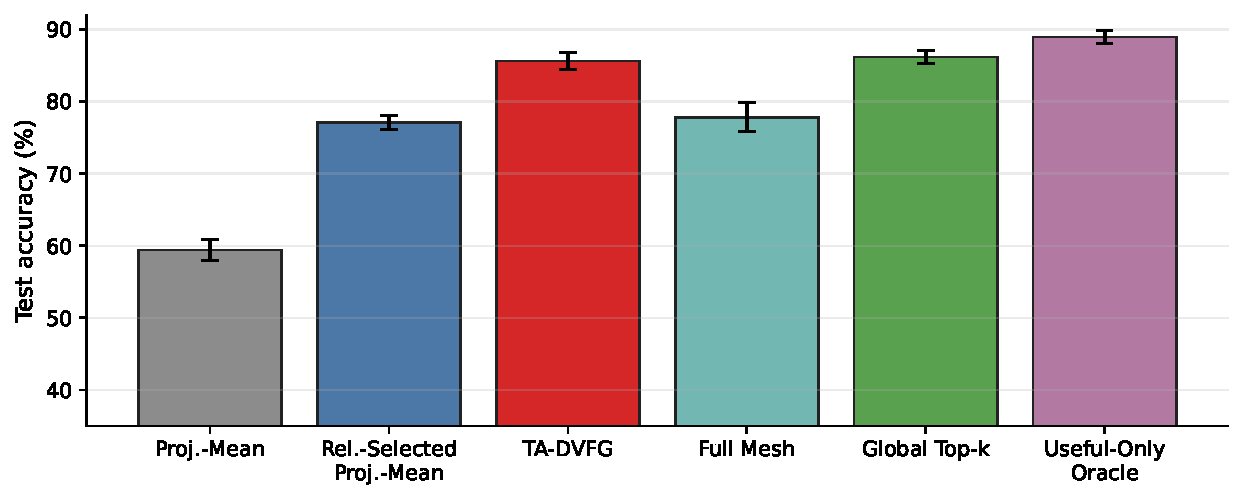
\includegraphics[draft=false,height=0.18\textheight,keepaspectratio]{figures/alignment_acmhard5_five_seed.pdf}\hfill
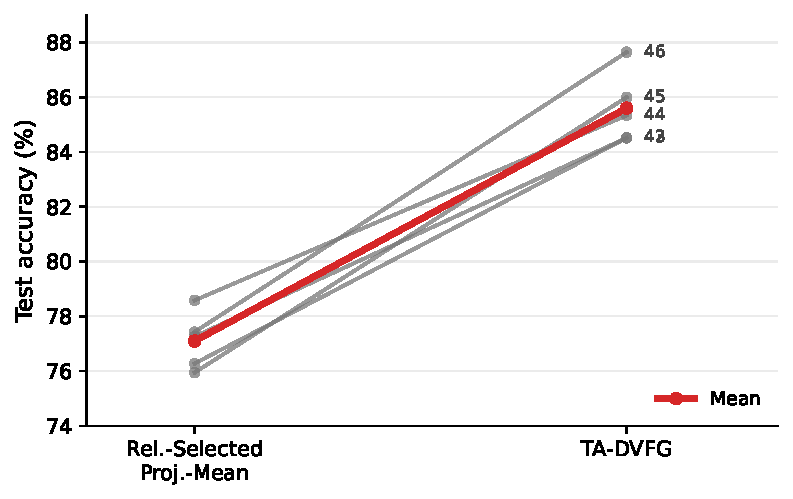
\includegraphics[draft=false,height=0.18\textheight,keepaspectratio]{figures/alignment_acmhard5_paired_lines.pdf}
\caption{ACM Hard alignment-reference diagnostics. Left: five-seed mean
performance with one-standard-deviation error bars; the useful-only latent row
is an oracle diagnostic. Right: paired per-seed comparison between
Reliability-Selected Project-and-Mean and \method{} on identical frozen local
predictors.}
\label{fig:supp-alignment-diagnostics}
\end{figure*}

\paragraph{Party-selection diagnostic.}
Reliability-selected latent fusion selects all three useful parties and two weak
parties in every seed. The useful-only oracle removes those two weak selected
parties and reaches $88.93\pm0.94\%$, showing that latent fusion is not
intrinsically weak when useful-party identities are known. The deployable
difficulty is selecting and combining parties without that oracle information.

\paragraph{Capability and payload boundaries.}
Table~\ref{tab:supp-alignment-boundaries} separates hidden-state collection,
prediction collection, and peer exchange. The latent references require
centralized hidden-state collection and a shared projection interface.
\method{} never collects hidden states: consensus exchange is sparse P2P, an
active readout may collect post-consensus predictions, and party-local readout
requires no global collection.

\begin{table*}[!t]
\centering
\caption{Interface and payload-accounting boundaries for the ACM Hard alignment
references. Hidden payload is vector width per target; prediction payload is
total transmitted prediction scalars per inference run. The two payload columns
use different natural units and are not intended as a direct byte-for-byte
comparison.}
\label{tab:supp-alignment-boundaries}
\scriptsize
\textbf{Capability boundary}\\[2pt]
\begin{tabular}{lccccc}
\toprule
Method & Hidden-state collection & Prediction collection & Shared proj. & Sparse P2P & Party-local readout \\
\midrule
Global Top-$k$ & No & Yes & No & No & No \\
\method{} & No & Active readout only & No & Yes & Yes \\
Reliability-Selected P\&M & Yes & No & Yes & No & No \\
Useful-Only latent fusion (oracle) & Yes & No & Yes & No & No \\
\bottomrule
\end{tabular}

\vspace{5pt}
\textbf{Payload and trainable fusion parameters}\\[2pt]
\begin{tabular}{lrrrr}
\toprule
Method & Hidden width/target & Prediction payload/run & Fusion params & Hidden train cache \\
\midrule
Global Top-$k$ & 0 & 45,375 & 0 & 0 \\
\method{} & 0 & 90,750 & 0 & 0 \\
Reliability-Selected P\&M & 160 & 0 & 10,819 & 968,000 \\
Project-and-Mean & 480 & 0 & 32,259 & 2,904,000 \\
Useful-Only latent fusion (oracle) & 96 & 0 & 6,531 & 580,800 \\
\bottomrule
\end{tabular}
\end{table*}

\section{MovieLens Supplementary Evaluation}
\label{sec:supp-movielens}

MovieLens complements the controlled HGB suite with explicitly heterogeneous
predictors over aligned real-data recommendation targets. All MovieLens values
reported below come from the leakage-safe rerun with train-only timestamp
normalization. We use GroupLens
MovieLens 1M (\texttt{ml-1m.zip}) and the exact observed-rating task construction
defined above: rating $\ge4$ is positive, ratings $1$--$3$ are negative,
unobserved pairs are excluded, and no negative sampling is used. Rows are
ordered by \texttt{(timestamp, user\_id, movie\_id)} and split chronologically
70/10/20. The five-party experiment uses distinct private views and predictor
families, while the 15-party Main and Hard variants are controlled weak-predictor
stress settings. All parties score the same ordered aligned rating rows,
ROC-AUC is the task metric, and all reported results use seeds 42--46. All
model fitting, feature statistics, and timestamp normalization are train-only;
validation is reserved for reliability/topology selection and test labels for
final reporting.

\begin{table}[!t]
\centering
\footnotesize
\setlength{\tabcolsep}{3.5pt}
\caption{Five-party MovieLens predictor interfaces.}
\label{tab:supp-movielens-interfaces}
\begin{tabular}{cll}
\toprule
Party & Private view & Predictor family \\
\midrule
$P_1$ & Rating interactions & Matrix factorization \\
$P_2$ & User profiles & MLP \\
$P_3$ & Popularity / temporal & MLP \\
$P_4$ & Movie metadata & MLP \\
$P_5$ & Genre similarity & KNN-augmented MLP \\
\bottomrule
\end{tabular}
\end{table}

\begin{table*}[!t]
\centering
\caption{MovieLens summary over seeds 42--46. Left: five-party comparison,
including no-collaboration and centralized references. Right: controlled
15-party weak-predictor stress settings.}
\label{tab:supp-movielens-summary}
\begin{minipage}[t]{0.43\textwidth}
\centering
\footnotesize
\textbf{Five-party comparison}\\[2pt]
\resizebox{\linewidth}{!}{%
\begin{tabular}{lrr}
\toprule
Method & ROC-AUC & Total communication \\
\midrule
Best Single & 0.7402 & 0.00M \\
Global Top-$k$ & 0.7487 & 0.80M \\
Adaptive Pairwise & 0.7510 & 5.20M \\
Full Mesh & 0.7497 & 10.00M \\
\method{} & \textbf{0.7516} & 3.20M \\
\bottomrule
\end{tabular}%
}
\end{minipage}
\hfill
\begin{minipage}[t]{0.54\textwidth}
\centering
\footnotesize
\textbf{Fifteen-party Main/Hard stress settings}\\[2pt]
\resizebox{\linewidth}{!}{%
\begin{tabular}{lrrrr}
\toprule
Method & Main AUC & Main links & Hard AUC & Hard links \\
\midrule
Adaptive Pairwise & 0.7460 & 14.2 & 0.7433 & 14.0 \\
Full Mesh & 0.7455 & 105.0 & 0.7427 & 105.0 \\
\method{} & \textbf{0.7516} & \textbf{5.2} & \textbf{0.7498} & \textbf{5.0} \\
\bottomrule
\end{tabular}%
}
\end{minipage}
\end{table*}

\paragraph{Five-party comparison.}
Table~\ref{tab:supp-movielens-summary} includes Best Single at zero
communication. Its lower mean AUC than the collaborative methods shows that the
five-party result is not only a communication reduction relative to dense
exchange; prediction-level collaboration also improves over independent local
inference. The five predictors differ in private view, model family, parameter
count, validation ROC-AUC, test ROC-AUC, and validation--test generalization
gap. Exact parameter counts are included in the submitted code/data package.

\paragraph{Fifteen-party stress settings.}
These controlled settings support the narrower claim that sparse graph-level
selection is useful when many weak predictors are available. By themselves,
they do not establish a monotonic law over noisy-party count; that question is
tested separately by the nested HGB scaling study. The direct latent-alignment
study is likewise limited to ACM Hard and frozen local predictors and should
not be read as evidence that prediction-space collaboration universally
dominates every possible latent interface.

\section{Additional Protocol and Efficiency Audits}

\paragraph{Active-party validation and label location.}
Table~\ref{tab:supp-active-label-audits} first restricts validation reliability
and topology scoring to the active party with direct label access while reusing
the supervised cached predictors from the shuffled HGB core. Its second panel
also restricts direct training-label access: passive parties send train-node
logits and receive logit-space gradients. Because exact gradients can reveal
label information, this is a label-location/API-separation audit rather than a
label-confidentiality guarantee. Individual matched sparse controls remain in
Table~\ref{tab:supp-complete}; no post-hoc best-matched aggregate is used in
these protocol tables.

\begin{table*}[!t]
\centering
\caption{Active-party validation and label-location training audits. All values
are Test@BestVal accuracy (\%, mean $\pm$ standard deviation). Individual
matched sparse controls are reported separately in Table~\ref{tab:supp-complete};
no post-hoc best-matched aggregate is used here.}
\label{tab:supp-active-label-audits}
\scriptsize
\textbf{Active-party validation over seeds 42--46}\\[2pt]
\begin{tabular}{lccccr}
\toprule
Setting & \method{} & Global Top-$k$ & Full Mesh & $\Delta$ Full & Links \\
\midrule
ACM Main & $89.92\pm1.54$ & $89.82\pm1.01$ & $85.96\pm2.30$ & $+3.95$ & $5.2$ \\
ACM Hard & $86.99\pm2.73$ & $85.50\pm2.78$ & $75.52\pm5.04$ & $+11.47$ & $5.2$ \\
DBLP Main & $91.72\pm1.05$ & $91.43\pm0.65$ & $90.86\pm0.49$ & $+0.86$ & $5.6$ \\
DBLP Hard & $90.25\pm1.12$ & $90.57\pm1.04$ & $88.01\pm1.45$ & $+2.24$ & $5.2$ \\
\bottomrule
\end{tabular}

\vspace{5pt}
\textbf{Hard-setting label-location training}\\[2pt]
\begin{tabular}{lccc}
\toprule
Dataset & \method{} & Global Top-$k$ & Full Mesh \\
\midrule
ACM & $86.79\pm2.20$ & $85.83\pm2.33$ & $76.21\pm4.24$ \\
DBLP & $89.78\pm0.98$ & $90.49\pm1.02$ & $87.69\pm1.31$ \\
\bottomrule
\end{tabular}
\end{table*}

\paragraph{Deployment readout objectives.}
Tables~\ref{tab:supp-objective-acm} and
\ref{tab:supp-objective-dblp} compare active, party-local, and joint topology
objectives under the strict label-location protocol. They use the same all-party
local-mean definition and therefore form the primary deployment-objective audit.

\begin{table*}[!t]
\centering
\scriptsize
\setlength{\tabcolsep}{3pt}
\caption{ACM Hard readout-objective topology results under the strict
active-party label-location protocol. Communication entries are
peer/readout/control scalars; bold values denote the best result within each
metric.}
\label{tab:supp-objective-acm}
\begin{tabular}{llccrl}
\toprule
Method & Objective & Active & Local mean & Edges & Peer / Readout / Control \\
\midrule
Active Local Only & active & $34.99\pm1.33$ & $37.83\pm3.75$ & 0.0 & 0 / 0 / 0 \\
Global Top-$k$ & active & $85.77\pm2.27$ & $41.19\pm1.16$ & 0.0 & 0 / 45,375 / 0 \\
Full Mesh & active & $76.14\pm4.98$ & $43.07\pm0.89$ & 105.0 & 1,905,750 / 136,125 / 0 \\
\method{}-active & active & $86.89\pm2.26$ & $43.68\pm0.45$ & 5.0 & 90,750 / 50,820 / 203,850 \\
\method{}-local & local & $84.74\pm2.14$ & $43.85\pm0.35$ & 6.6 & 119,790 / 81,675 / 203,850 \\
\method{}-joint-$0.25$ & joint & $86.43\pm1.95$ & $\mathbf{43.94\pm0.33}$ & 5.0 & 90,750 / 47,190 / 203,850 \\
\method{}-joint-$0.50$ & joint & $\mathbf{86.99\pm2.19}$ & $43.79\pm0.45$ & 5.0 & 90,750 / 47,190 / 203,850 \\
\method{}-joint-$0.75$ & joint & $86.85\pm2.38$ & $43.80\pm0.46$ & 5.2 & 94,380 / 49,005 / 203,850 \\
\bottomrule
\end{tabular}
\end{table*}

\begin{table*}[!t]
\centering
\scriptsize
\setlength{\tabcolsep}{3pt}
\caption{DBLP Hard readout-objective topology results under the strict
active-party label-location protocol. Bold and underlined values denote the best
and second-best results within each metric.}
\label{tab:supp-objective-dblp}
\begin{tabular}{llccrl}
\toprule
Method & Objective & Active & Local mean & Edges & Peer / Readout / Control \\
\midrule
Active Local Only & active & $27.05\pm1.33$ & $31.35\pm2.34$ & 0.0 & 0 / 0 / 0 \\
Global Top-$k$ & active & $\mathbf{90.20\pm1.26}$ & $33.33\pm0.54$ & 0.0 & 0 / 81,140 / 0 \\
Full Mesh & active & $87.44\pm1.74$ & $37.73\pm0.45$ & 105.0 & 3,407,880 / 243,420 / 0 \\
\method{}-active & active & $89.80\pm1.07$ & $35.95\pm1.45$ & 5.2 & 168,771 / 110,350 / 363,600 \\
\method{}-local & local & $89.43\pm1.67$ & $\mathbf{38.76\pm0.39}$ & 7.6 & 246,666 / 165,526 / 363,600 \\
\method{}-joint-$0.25$ & joint & $\underline{90.15\pm1.38}$ & $\underline{38.45\pm0.42}$ & 6.0 & 194,736 / 133,070 / 363,600 \\
\method{}-joint-$0.50$ & joint & $89.95\pm1.40$ & $38.25\pm0.76$ & 5.4 & 175,262 / 120,087 / 363,600 \\
\method{}-joint-$0.75$ & joint & $89.88\pm1.11$ & $37.63\pm0.68$ & 5.4 & 175,262 / 103,859 / 363,600 \\
\bottomrule
\end{tabular}
\end{table*}

\paragraph{Communication accounting.}
Table~\ref{tab:supp-communication} separates peer exchange from readout payload.
The active-readout configuration counts both terms; a party-local readout would
incur no additional global readout collection. Under the benchmark accounting,
\method{} reduces total deployment communication from 2.04M to 0.15M scalars
relative to Full Mesh. HGB and MovieLens communication totals should not be
mixed numerically because they use different target counts and task protocols.

\begin{table}[!t]
\centering
\footnotesize
\caption{ACM Main benchmark communication accounting (scalars).}
\label{tab:supp-communication}
\begin{tabular}{lrrr}
\toprule
Method & Peer & Readout payload & Total \\
\midrule
Global Reliability & 0 & 136,125 & 136,125 \\
Global Top-$k$ & 0 & 45,375 & 45,375 \\
Full Mesh & 1,905,750 & 136,125 & 2,041,875 \\
\method{} & 90,750 & 61,710 & 152,460 \\
\bottomrule
\end{tabular}
\end{table}

\paragraph{Topology-label and update-frequency efficiency.}
Figure~\ref{fig:supp-label-budget} reports topology-label budget and
update-frequency sensitivity. Using fewer topology labels or updating less
frequently reduces control traffic without changing the qualitative conclusion.

\begin{figure*}[!t]
\centering
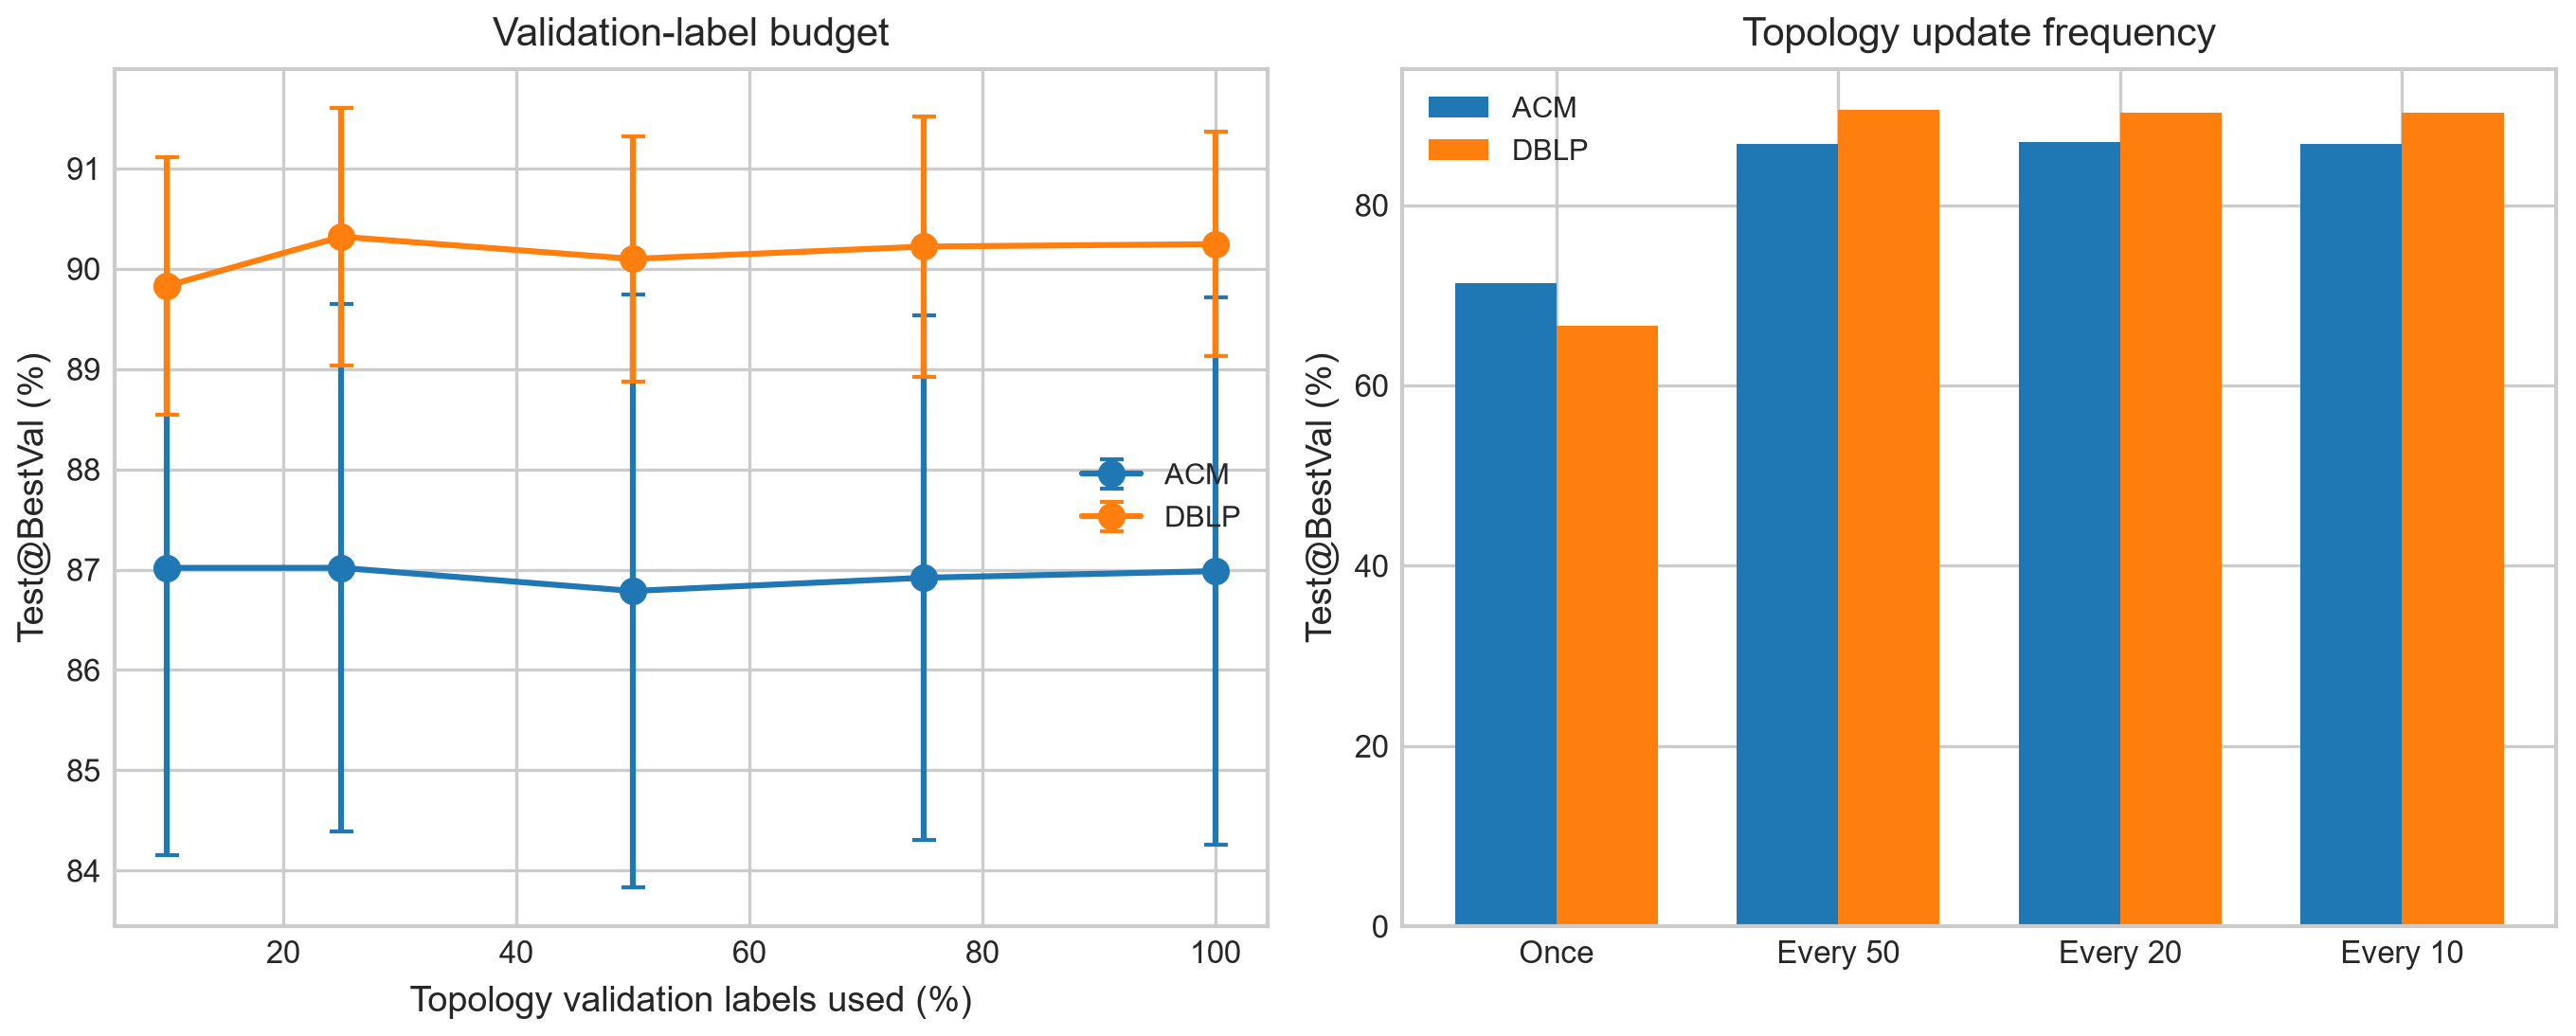
\includegraphics[width=0.60\textwidth]{figures/label_budget_topology_frequency_tight.png}
\caption{Validation-label budget and topology-update frequency under active-party
topology selection.}
\label{fig:supp-label-budget}
\end{figure*}

\paragraph{Scalability.}
Table~\ref{tab:supp-scalability} shows that selected graphs remain near five
links from 5 to 30 parties, while candidate evaluations and topology-selection
time grow much faster. This identifies exhaustive candidate scoring, rather
than sparse deployment, as the principal scalability bottleneck.

\begin{table}[!t]
\centering
\footnotesize
\caption{ACM Hard party-count scalability with a fixed 20\% useful-party ratio.}
\label{tab:supp-scalability}
\begin{tabular}{rrrrrr}
\toprule
Parties & Useful & Test@BestVal & Links & Evals & Time (s) \\
\midrule
5  & 1 & $82.73\pm1.64$ & 5.0 & 617 & 0.81 \\
10 & 2 & $84.32\pm0.96$ & 5.0 & 3,560 & 5.21 \\
15 & 3 & $86.26\pm2.35$ & 5.0 & 8,996 & 13.93 \\
20 & 4 & $88.11\pm1.17$ & 5.4 & 17,358 & 30.39 \\
30 & 6 & $87.87\pm2.20$ & 5.0 & 41,542 & 81.46 \\
\bottomrule
\end{tabular}
\end{table}

\section{Selector and Consensus Sensitivity}

\paragraph{Minimum-link requirement.}
The headline configuration uses $m=5$, but collaboration does not depend on
that quota. With $m=0$, the implementation permits the edgeless topology and
accepts the first edge only when its validation gain clears $\tau$. Nevertheless,
all five seeds on both Hard datasets select nonempty graphs, as summarized in
Table~\ref{tab:supp-minlink-audit}. DBLP performance is unchanged relative to
the existing $m=5$ sweep, while ACM is higher in that sweep. Thus, nonempty
sparse collaboration emerges without a forced minimum.

\begin{table}[!t]
\centering
\scriptsize
\setlength{\tabcolsep}{3.0pt}
\caption{Minimum-link audit with $m=0$. Edge counts follow seeds 42--46;
first-edge gains are validation-score improvements over the edgeless graph.}
\label{tab:supp-minlink-audit}
\begin{tabular}{lcccc}
\toprule
Dataset & Edges by seed & Mean & Empty seeds & First-edge gain \\
\midrule
ACM Hard & 3, 3, 2, 2, 3 & 2.6 & 0/5 & $[0.0480,\,0.1821]$ \\
DBLP Hard & 3, 3, 4, 3, 2 & 3.0 & 0/5 & $[0.0284,\,0.0407]$ \\
\bottomrule
\end{tabular}
\end{table}

\paragraph{Consensus components.}
Figure~\ref{fig:supp-consensus} tests consensus depth, self-weight, uniform
weighting, and reliability weighting. The \texttt{steps0} bars rerun the full
epoch-level pipeline and independently reselect topology with $K=0$; they are
not a fixed-topology no-message intervention. As shown in
Table~\ref{tab:supp-steps0-audit}, default and \texttt{steps0} have similar
active accuracy but select different graphs in every seed. The fixed-state
exchange effect is therefore reported separately in
Table~\ref{tab:supp-exchange-decomposition}.

\paragraph{Budget and gain threshold.}
Figure~\ref{fig:supp-edge-budget} shows that increasing the edge budget does not
force the selected graph to become dense. The gain threshold controls early
stopping, while the budget remains an upper bound rather than a quota.

\begin{figure*}[!t]
\centering
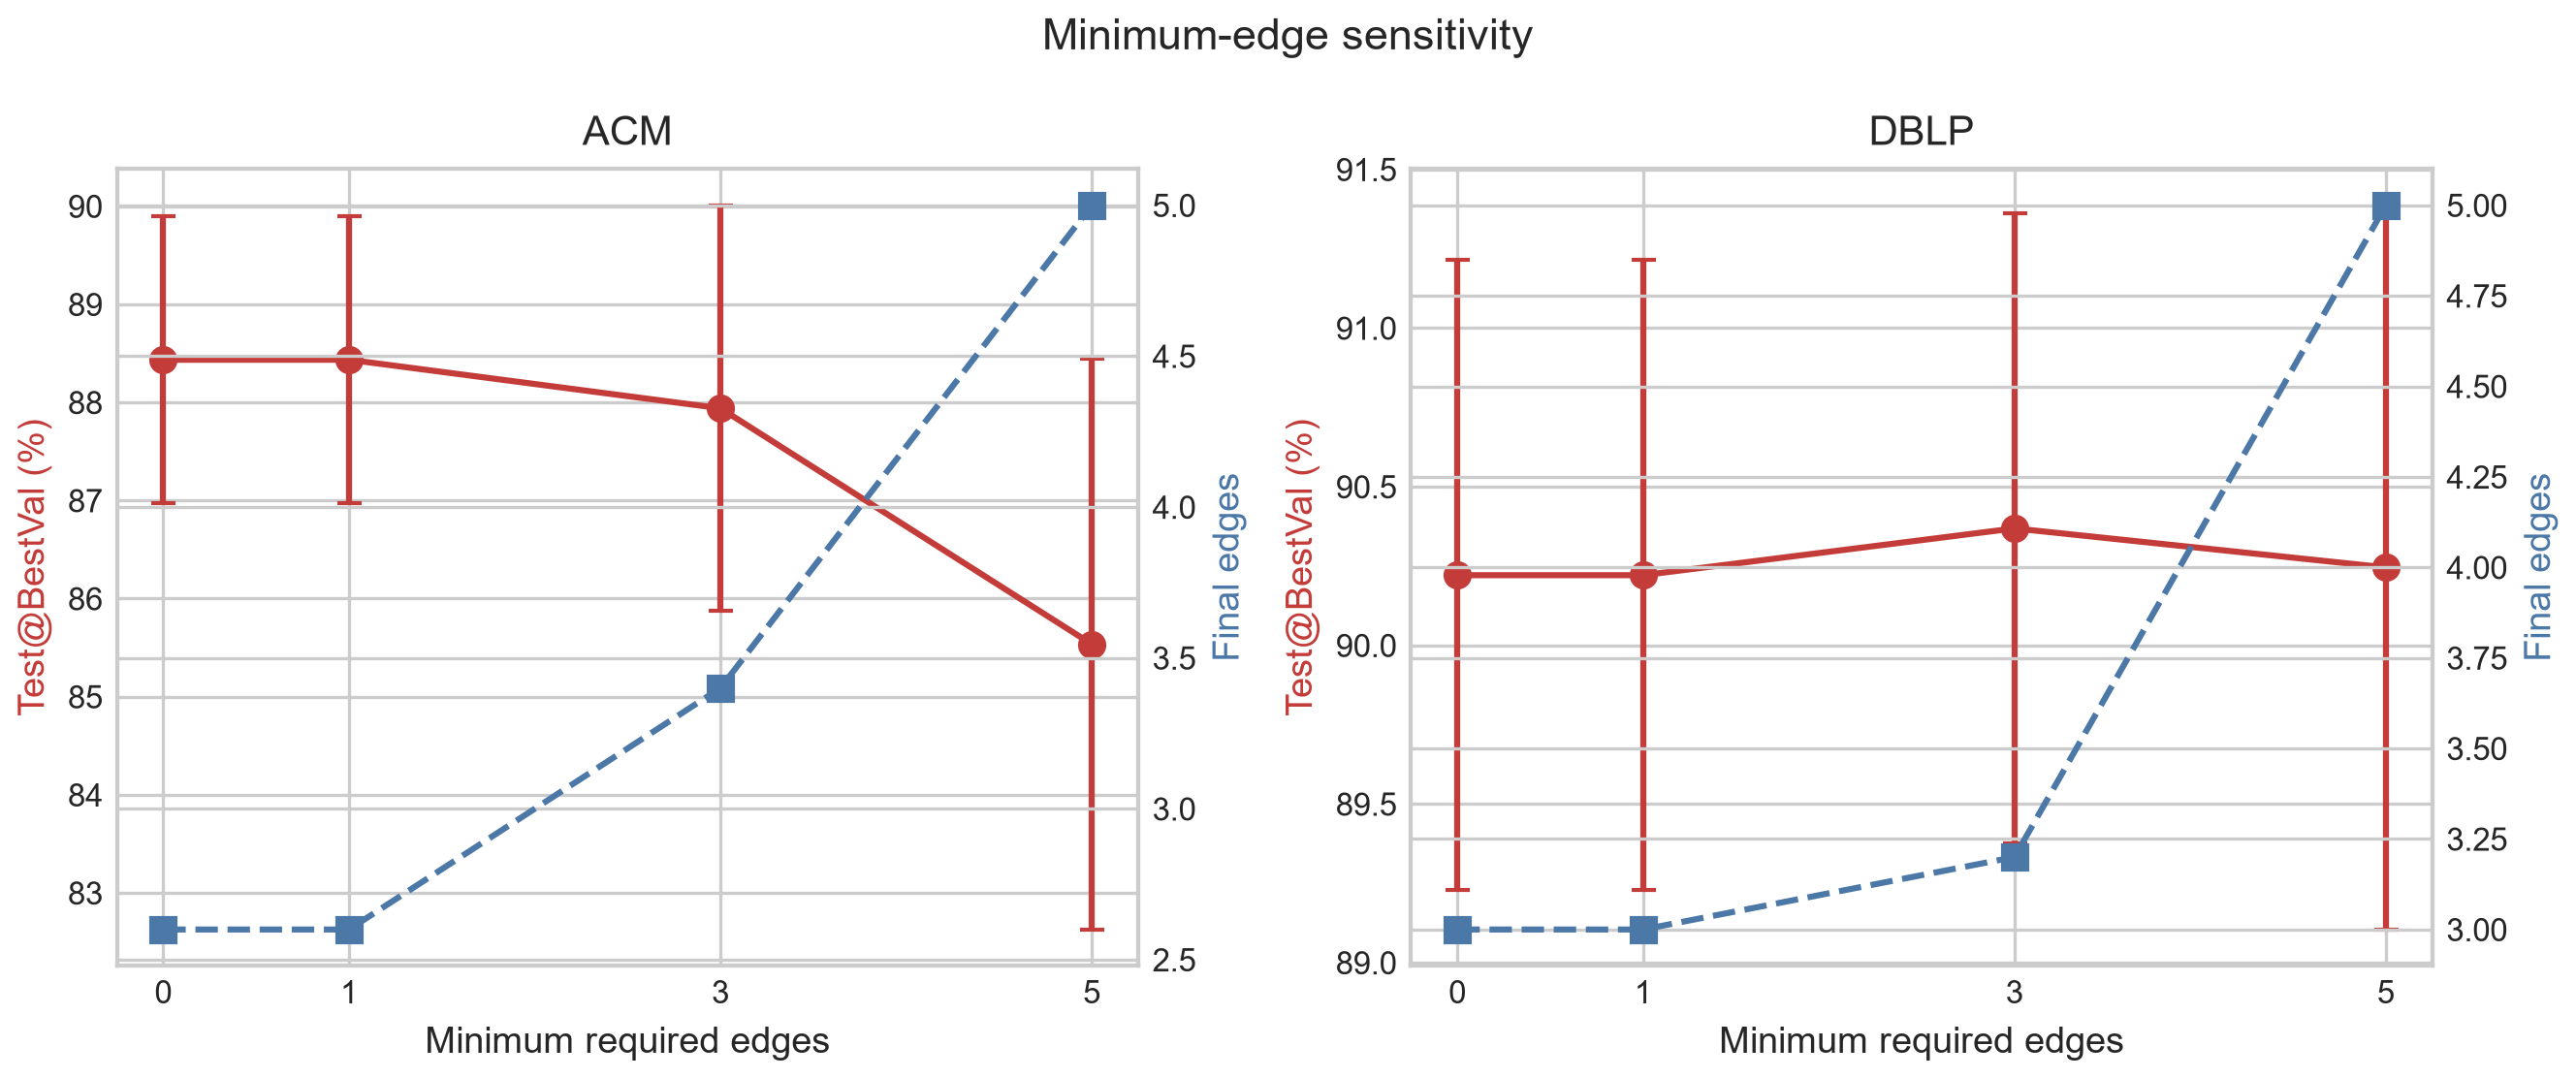
\includegraphics[width=0.75\textwidth]{figures/minedges_sensitivity_tight.png}
\caption{Minimum-link sensitivity for sparse P2P prediction consensus.}
\label{fig:supp-minedges}
\end{figure*}

\begin{figure*}[!t]
\centering
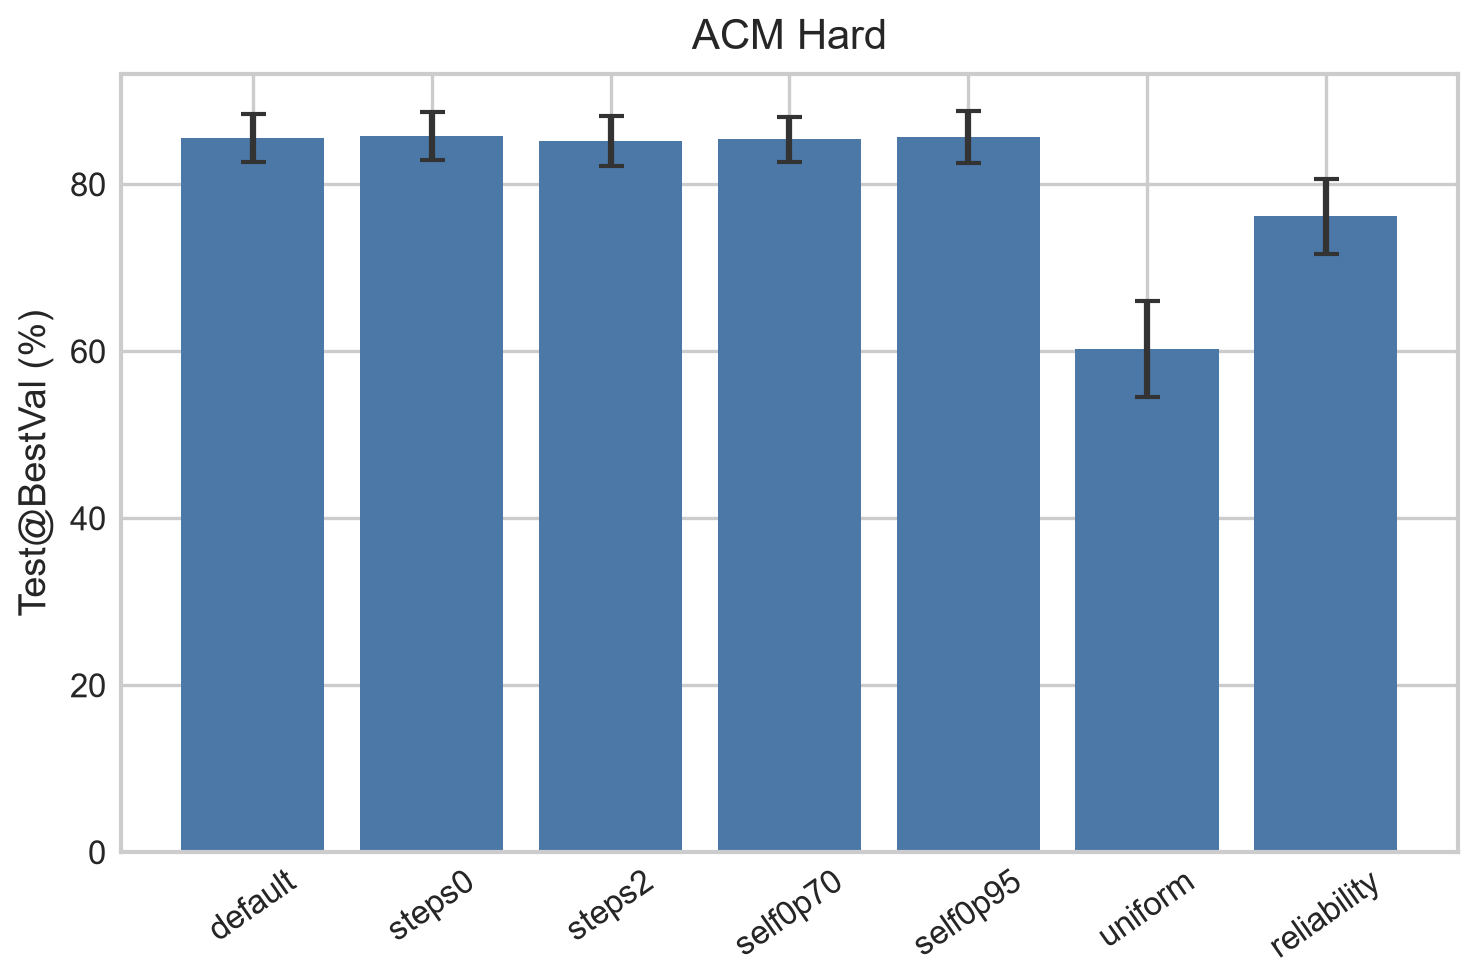
\includegraphics[width=0.40\textwidth]{figures/consensus_ablation_p11.png}\hfill
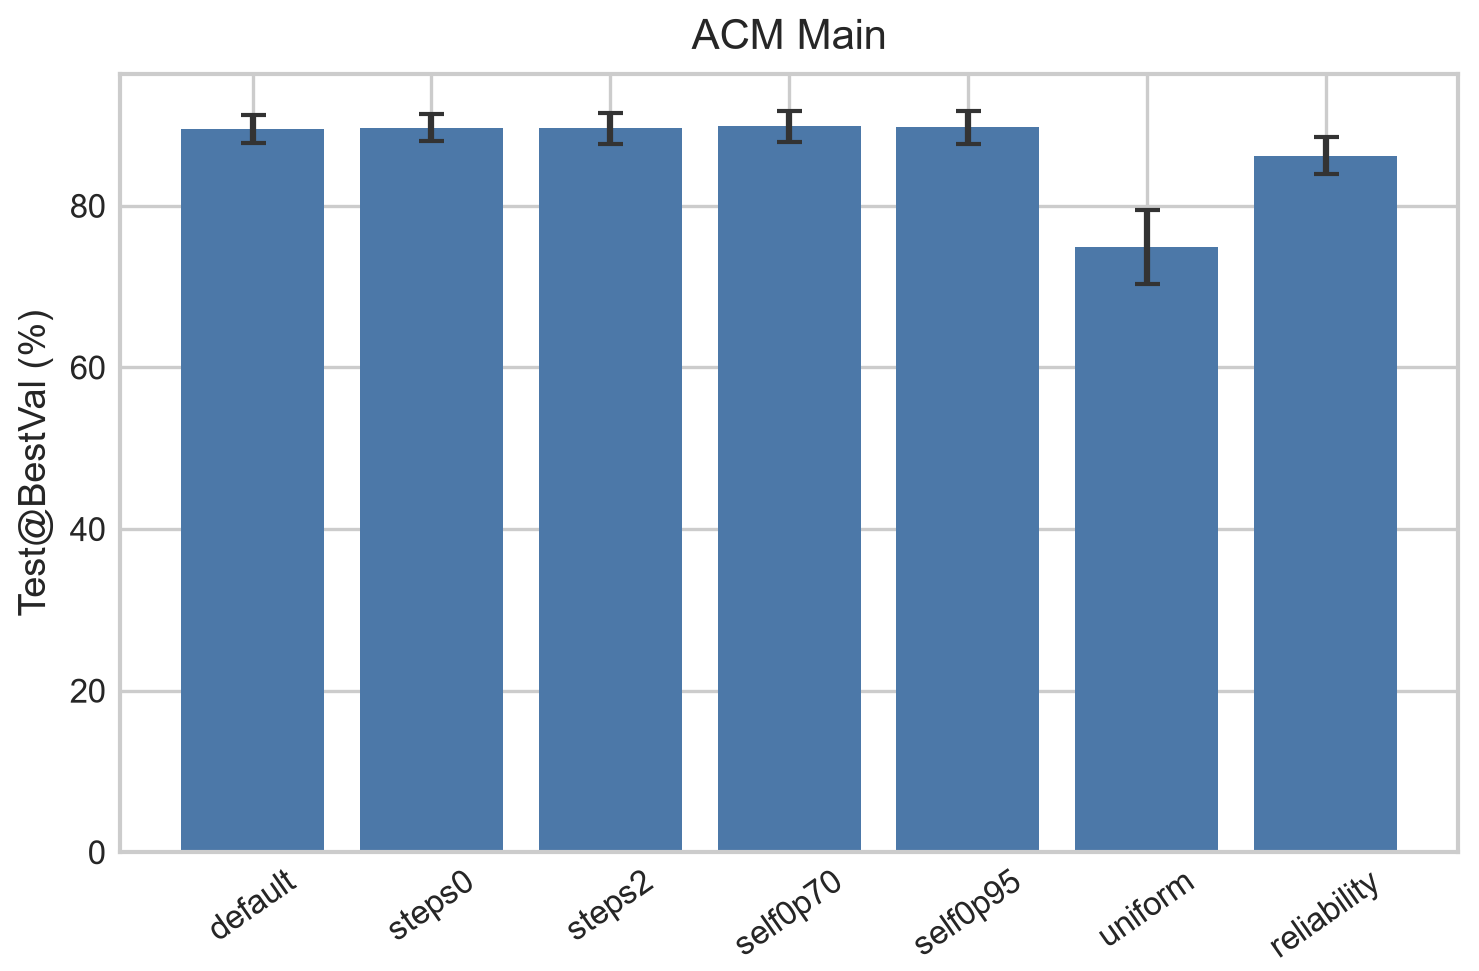
\includegraphics[width=0.40\textwidth]{figures/consensus_ablation_p12.png}
\vspace{2pt}
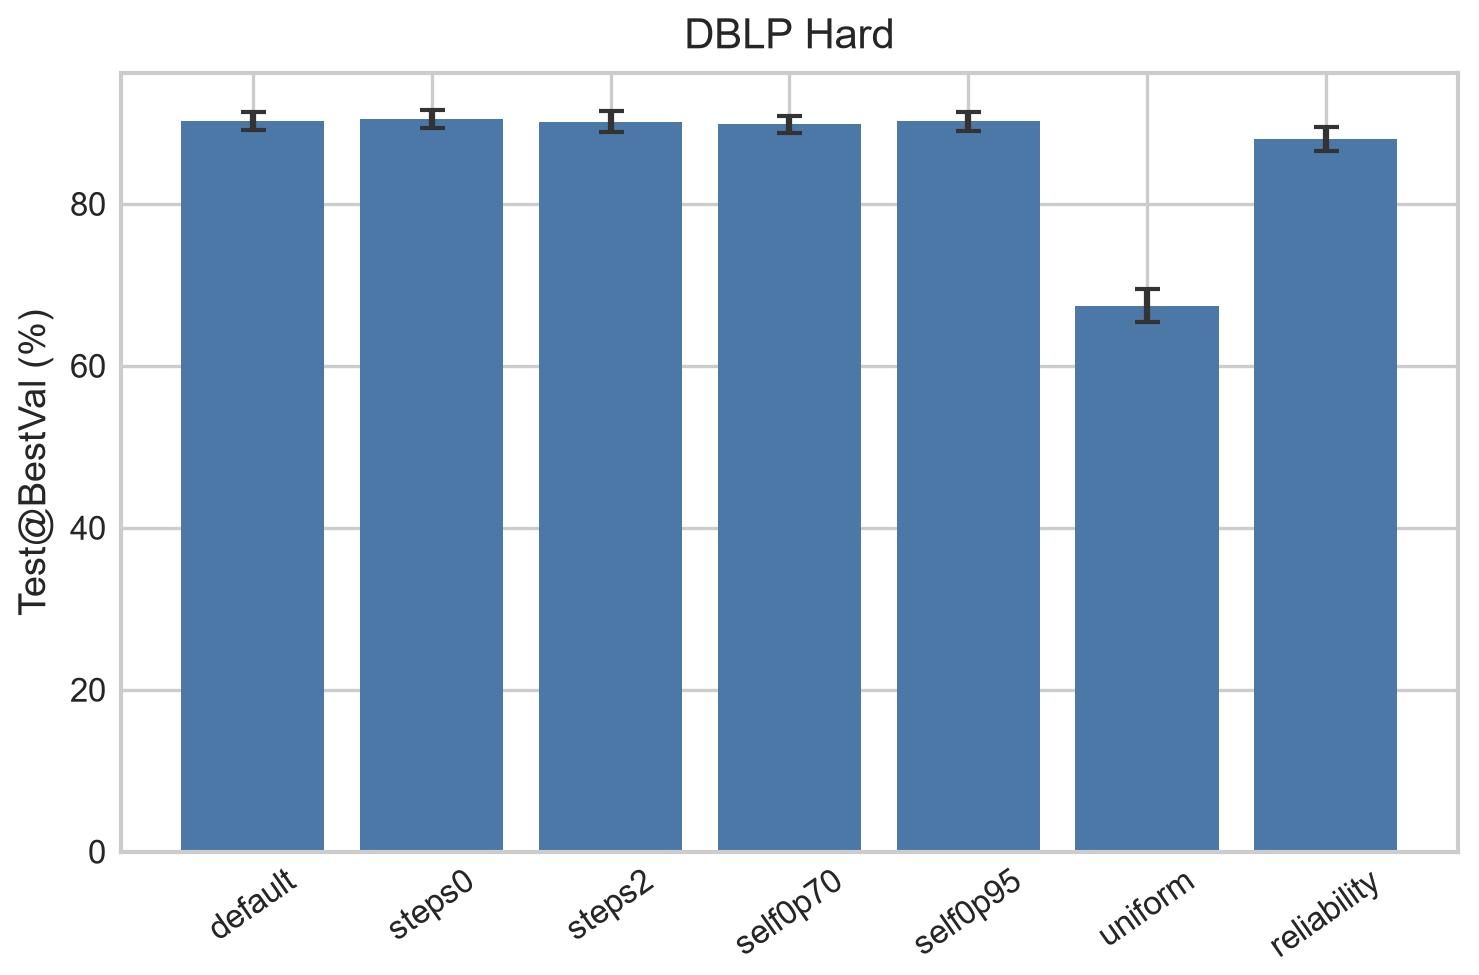
\includegraphics[width=0.40\textwidth]{figures/consensus_ablation_p21.png}\hfill
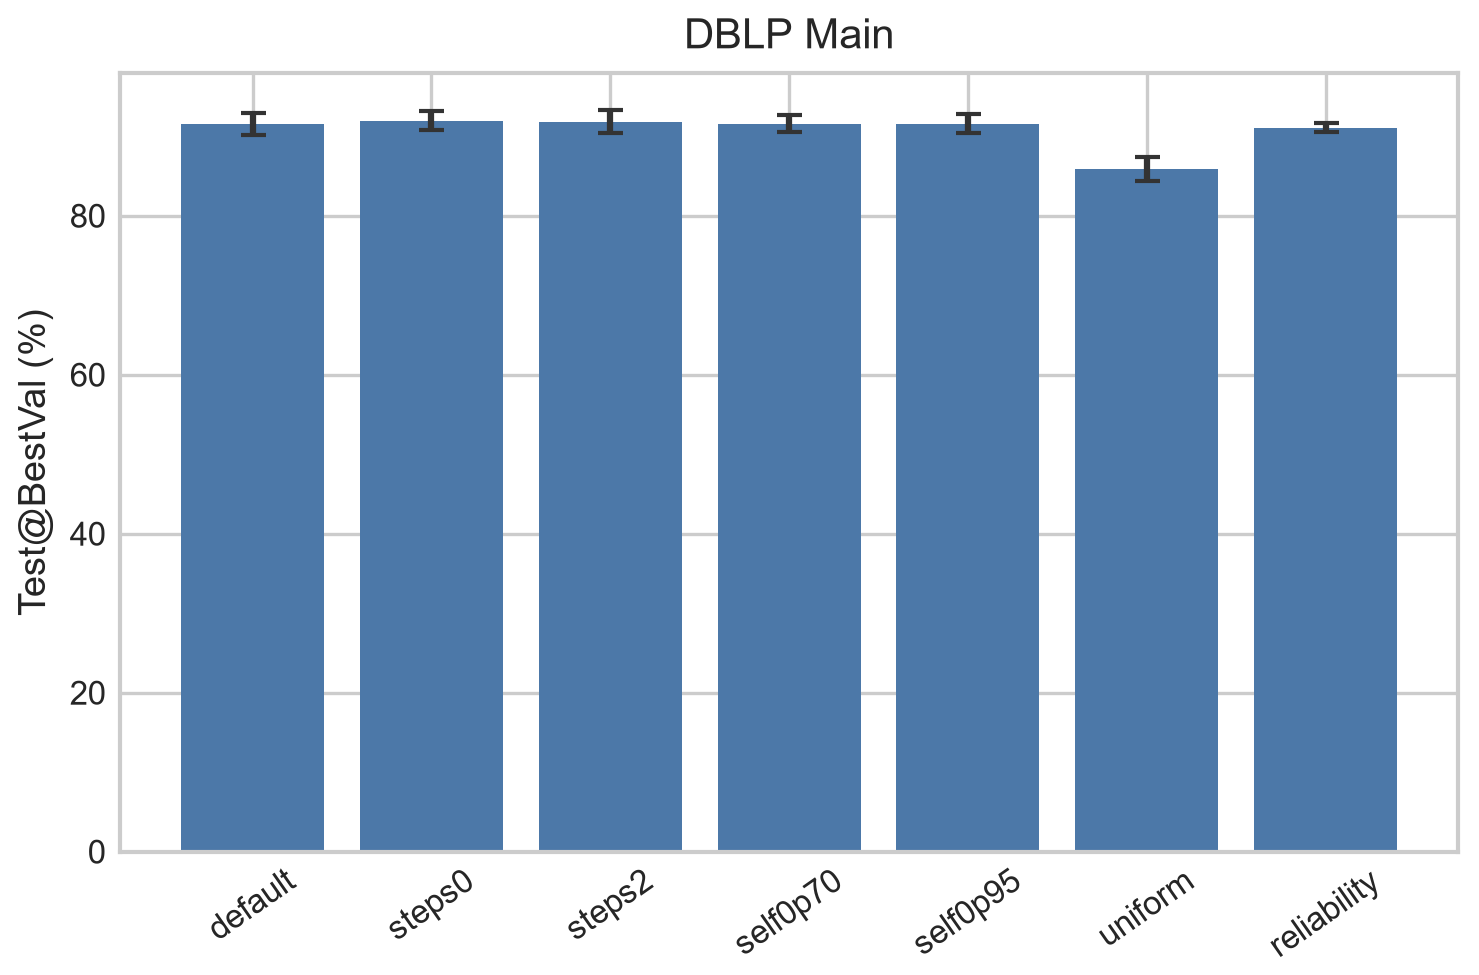
\includegraphics[width=0.40\textwidth]{figures/consensus_ablation_p22.png}
\caption{Consensus-step, self-weight, and reliability-weighting
ablations. The \texttt{steps0} condition independently reselects topology with
$K=0$ and should not be interpreted as a fixed-topology no-message
intervention.}
\label{fig:supp-consensus}
\end{figure*}

\begin{figure*}[!t]
\centering

\includegraphics[width=0.4\textwidth]{figures/edge_budget_acm_edges.pdf}\hfill

\includegraphics[width=0.4\textwidth]{figures/edge_budget_dblp_edges.pdf}
\caption{Selected-edge diagnostics for edge-budget sweeps on ACM and DBLP.}
\label{fig:supp-edge-budget}
\end{figure*}

\section{Statistical Reporting}

All primary HGB and MovieLens results use seeds 42--46. Reported
mean--dispersion summaries follow the same five-seed aggregation convention as
the main paper. Paired tests compare methods or protocol variants under shared
seeds and matched experimental conditions. The HGB analysis reports paired
$t$-tests, Wilcoxon signed-rank tests, 95\% confidence intervals, paired
Cohen's $d_z$, and Holm correction. With five seeds, confidence intervals and
effect sizes should be read alongside $p$-values rather than as standalone
guarantees.

For MovieLens, the submitted supplementary package contains paired statistics
and per-seed AUC/communication deltas for the five-party Pareto analysis.
Because the mean AUC margins are small, the main paper emphasizes communication
reduction and paired trade-off evidence rather than a large accuracy-gain
claim. The 15-party Main and Hard results are controlled stress settings, not
evidence for a universal monotonic law over noisy-party count.

For the ACM Hard alignment-reference study, the primary paired comparison is
Reliability-Selected Project-and-Mean minus \method{}: $-8.50$ points with
95\% CI $[-10.47,-6.54]$, paired $t$-test
$p=2.76\times10^{-4}$, and win/tie/loss $0/0/5$. The useful-only latent-fusion
result is an oracle diagnostic and is excluded from deployable-baseline claims.

The HGB label-location versus supervised differences are $-0.20$ points on ACM
and $-0.47$ on DBLP and are not significant. Topology-label budget and
10/50-versus-20-epoch update-interval comparisons are also not significant
after Holm correction. Fully local readouts remain substantially below the
active readout under paired tests.

For the mechanism audit, the primary inferential result is the same-state
peer-exchange intervention. Active differences are small and non-significant
($p=.3046/.1778$ on ACM/DBLP), whereas all-party local-mean improvements are
1.85 and 2.67 points with paired $p=.002244$ and
$6.677\times10^{-5}$. The direct degree-factor effects are also small
($p=.08016/.298$). Same-cardinality subset baselines match or slightly exceed
\method{} in mean active accuracy, but the paired accuracy differences are not
significant; their communication reductions relative to \method{} are strongly
significant under the same five seeds. These results support an
interface-dependent mechanism claim rather than an equivalence claim.

For the consensus-depth study, the primary interpretation is descriptive:
predictive performance remains stable while $K$-hop reachability expands.
Because peer communication scales linearly with $K$, deeper consensus is not
treated as beneficial unless the additional reach is required.

For nested weak-party scaling, we emphasize paired mean differences,
win/tie/loss counts, and the widening effect-size trend across the controlled
sequence. With only five seeds, the minimum attainable two-sided exact
Wilcoxon value under five nonzero differences is 0.0625; non-significance is
therefore not interpreted as evidence against the observed effect-size trend.

\section{Reproducibility Notes}

\paragraph{HGB data construction.}
The HGB cached core, active-party validation, label-budget,
topology-frequency, label-location-training, scalability, and selector-sensitivity
studies use seed-dependent shuffled useful/noisy positions. All parties retain
the same aligned target nodes, labels, and dataset-level train/validation/test
split. Useful parties use the stated metapath/KNN views. For every weak/noisy
party, the private feature rows are permuted with a seed-specific permutation,
zero-mean Gaussian noise of scale $1.0$ is added, and the private graph is
replaced by an independently sampled random graph with configured degree $4$.
The resulting party identities are reshuffled again per seed. Protocol sweeps
that do not retrain local models reuse the same cached local trajectories as the
core; strict label-location training and scalability use dedicated caches.

\paragraph{MovieLens 1M task construction and leakage control.}
The MovieLens suite uses the GroupLens MovieLens 1M release
(\texttt{ml-1m.zip}). Targets are observed rating rows rather than unobserved
user--item pairs. Ratings $\ge4$ are positive, ratings $1$--$3$ are negative,
and no negative sampling is performed. Rows are ordered by
\texttt{(timestamp, user\_id, movie\_id)} and split chronologically into
70\%/10\%/20\% train/validation/test partitions. All five parties use the same
ordered target rows. Matrix factorization, all local predictors, popularity,
mean-rating, positive-rate and count statistics, and timestamp-normalization
mean/standard deviation are fit on training rows only. Validation labels are
used only for reliability estimation and topology selection; test labels are
used only for final reporting.

The MovieLens suite is implemented by
\path{experiments/movielens/run_movielens_tadvfg.py},
\path{prepare_movielens.py}, \path{plot_movielens_results.py},
\path{extended_movielens_suite.py}, \path{aggregate_15party.py}, and
\path{package_final_results.py}, together with
\path{models/movielens_parties.py}. The submitted code/data package contains
main-text figures, supplementary figures, raw CSV/JSON outputs, scripts, and a
usage README. The five-party suite covers ten methods; the 15-party Main/Hard
suite uses six useful plus nine weak parties and three useful plus twelve weak
parties, respectively, with Full Mesh verified as 105 undirected edges.

The headline HGB configuration was audited at run level: all 90 audited rows
resolve to $m=5$, $\tau=0.001$, $B=15$, $d_{\max}=2$, $K=1$, and
self-weight $\eta=0.85$. Consensus and active readout use
$\bar r_i=\max(r_i,10^{-3})$ with reliability exponent $1.0$. Active readout
additionally multiplies by $(\deg_E(i)+1)^{0.5}$ before normalization, uses
non-isolated parties whenever $E\neq\emptyset$, and falls back to all parties
only for the edgeless topology. The active party receives no special term.
The MovieLens wrapper parameter \texttt{final\_reliability\_floor=0.0} is a
separate wrapper-stage setting and is not the $10^{-3}$ floor used in the
consensus/readout weights.

\paragraph{Paper-evaluation state and topology provenance.}
The cached fields \texttt{probs\_val}/\texttt{probs\_test} are final local-model
snapshots and are not sufficient to reproduce Test@BestVal. The paper
evaluation uses \texttt{probs\_val\_epochs}/\texttt{probs\_test\_epochs},
replays the full epoch trajectory, refreshes adaptive topology every 20 epochs,
and records same-epoch test performance whenever validation improves. The
paper-evaluation replay reproduces all ten ACM/DBLP Hard headline runs within
float32/CPU tolerance.

The audit also identified a historical metadata mismatch: cached result CSVs
store final/last-refresh edge identities in \texttt{selected\_edges}, whereas
Test@BestVal may correspond to an earlier topology. The historical edge lists
match the replay final/last-refresh topology for all ten audited Hard runs. They
are therefore not used as ground truth for mechanism analysis. All Task 1--4
mechanism results use the paper-evaluation trajectory bundles and the topology
present at the selected best-validation state. In the audited ten runs, the
correction affects edge identity provenance, not Test@BestVal or the five-edge
count.

\paragraph{Mechanism-audit reproducibility.}
The $K=0$, fixed-state exchange, fixed-topology trajectory, degree-weighting,
and same-cardinality subset analyses reuse the same local prediction
trajectories and labels. Same-state interventions hold the epoch, topology,
participant set, degree vector, reliability vector, and prediction snapshot
fixed except for the explicitly ablated component. Direct subset baselines set
$q=|\mathcal{S}(E)|$ from the corresponding default topology state and use
validation labels only for ranking or greedy subset selection; test values are
evaluated only after selection. Historical CSV edge metadata is excluded from
all topology-identity checks.

The ACM Hard direct alignment-reference suite uses fresh frozen local predictors
and therefore remains separate from the historical cached-core tables. All 75
hidden-export equivalence checks pass. The suite includes all-party and
reliability-selected latent-fusion references plus a useful-only oracle
diagnostic. Broader multi-dataset or end-to-end latent-alignment studies and a
controlled architectural-heterogeneity ladder remain future work.

Across all regimes, \method{} should be read as an inference-stage
topology/readout mechanism: it avoids centralized hidden-representation fusion
and uses sparse P2P consensus, while active readout may still collect
post-consensus predictions. The mechanism audits further show that graph
learning is not required for the active-only interface, where direct subset
selection is a stronger lightweight alternative; the learned topology is
distinctly justified when party-local predictions must also improve through
peer exchange. The method is not a fully serverless end-to-end VFGL protocol
and not a formal privacy mechanism.

The consensus-depth study is implemented by
\path{run_k_sensitivity.py} under \path{experiments/} and reuses the audited
HGB prediction caches while rerunning topology selection independently for each
$K\in\{1,2,3\}$.

The nested weak-party study is implemented by
\path{run_nested_weak_scaling.py} under \path{experiments/}. Per seed, it fixes the useful-predictor core and evaluates nested subsets containing
0, 2, 5, 10, and 15 weak predictors.

\end{document}
